%%%%%%%%%%%%%%%%%%%%%%%%%%%
\chapter {Parallel Black Virus Decontamination in Meshes and Tori}
\label{DL}
%%%%%%%%%%%%%%%%%%%%%%%%%%%

In this Chapter, we discuss parallel strategies for the BVD problem in grids and tori. In the sequential strategy ({\em BVD-2G}) for 2-dimensional grids, an ``explorer agent'' and a ``leader explorer agent'' are sent to explore the graph and locate the BV. They traverse the mesh in a snake-like fashion, column by column, following   ``cautious walk''. In the sequential protocol ({\em BVD-qG}) for q-dimensional grids, the grid is partitioned into $d_1\times\ldots\times d_{q-2}$ 2-dimensional grids of size $d_{q-1}\times d_q$, and each 2-dimensional grid is explored using the shadowed traversal technique as described in the 2-dimensional grids. Similarly, in the protocol ($BVD-qT$) for q-dimensional torus, the torus is partitioned into $d_1\times \ldots \times d_{q-1}$ ring of size $d_q$. The exploration procedure traverses a ring and, when back to the starting point, proceeds to another ring, with a neighbouring starting point. After locating the BV, agents surround the new formed BVs sequentially and eliminate them. These strategies are simple to follow, but at the same time they are not time-efficient. We now consider the situation when  more than two agents are allowed to participate in the exploring phase and we focus on decreasing the time cost in the exploring phase and the number of casualties; that is, we focus on how to design a new strategy so that the we are able to reach the destination faster, but with  an acceptable cost in terms of number of agents.\\
\color{blue} at his point it is not clear what you mean by ``array", do you mean a compact area of consecutive/adjacent nodes ? I add the explanation below.
\color{black}
The general idea is simple, we will employ a group of agents and place them in a compact area of consecutive or adjacent nodes (for convenience, let us call it ``array") at the beginning.  Informally, in the shadowed exploration of our strategy in 2-dimensional grid({\em PBVD-2G}), q-dimensional grid ({\em PBVD-qG}) and tori ({\em PBVD-qT}), the agents that are employed to explore the graph stay in that array and this  ``array of agents"  traverse that graph in the shadowed exploration. 
Note that, after the BV is triggered, not all the agents automatically enter the elimination phase but only the ones that   know the existence of the  BV. However,  in some cases, the number of agents that know the existence of BV is not sufficient for surrounding and eliminating the BVs. For this reason,  in the elimination phase, our strategies employ some agents that know  the existence of the BV (because they receive the clones of the original BV) to notify some other agents to participate in the elimination phase as well. 
We study the number of agents, the time cost, the number of movements and  casualty, comparing them with  the ones of the corresponding sequential strategy.

\section{Parallel BV Decontamination of Grids}
\subsection{Base Case: 2-Dimensional Grid}
A 2-dimensional grid (which is a mesh) of size $d_1\times d_2$ has $n=d_1\times d_2 (d_1>2,d_2>2)$ nodes. Without loss of generality, let $d_1<d_2$ and let the nodes of {\em M} be denoted by their column and row coordinate ($x_1$,$x_2$), $1\leq x_1 \leq d_1$, $1\leq x_2 \leq d_2$. Observe that in a mesh, we have three types of nodes: \textit{corner} (entities with only two neighbours), \textit{border}(entities with three neighbours), and \textit{interior}(with four neighbours).  Our strategy follows two phases: shadowed exploration and elimination. In the first phase, the network is traversed until the location of the BV is determined. That location is found after the visit, at which time    all the  unprotected neighbours have become BVs.  Note that in $PBVD-2G$, there is  only one new formed BV. In the second phase, the new formed BV is surrounded and permanently eliminated. Note that when we say that  the second phase starts, we actually mean that those agents knowing the existence of BV start to surround the BV, or notify some other agents, and then eliminate the BV, but not   that all the agents enter this phase. There are two significant differences between $PBVD-2G$ and the sequential strategy: mainly the number of agents employed in the exploration phase and  the route of agents in the exploration phase. We also describe the routes of agents in the elimination phase. \ \\

\noindent{\bf Shadowed Exploration Phase} \\

As we mentioned above, we should place the agents in a specific array at the beginning and then let them explore the graph. Let us now   consider how to arrange them at the beginning and how to design the routes for them to explore the graph. We prefer to place the agents at the borders (or the corners) of the mesh because in this way we can reduce the casualties. For the same purpose of reducing the casualties, we prefer to arrange all the agents in an array so that when one of the exploring agent triggers the BV, the exploring agents and shadowed agents guide as many neighbours of the BV as possible. In other words, we want all the agents to explore the graph in one direction rather than   from different directions. With these two principles, our strategy in the shadowed exploration is the following:
 given a specific number of agents, we place them in one border of the mesh and if there are more agents, we place the extra agents in the next  row, and so on. Then we design routes for the agents so that at any time they move to the same direction to explore the graph. \\
Monotonicity is a principle that we should obey in the whole process, which means one exploring agent should be followed by at least one shadowed agent, so the number of agents in the exploration phase should be at least twice the number of the exploring agents. To guarantee the monotonicity and the two principles, we should employ $2a\,(a\in\mathbb{Z}^+)$ agents in this phase and place $a$ of them in one of the border and the others in the second line paralleling to the border.
Let us now consider the number of agents we should employ.
When $a=1$, the arrangement is actually the same as in the sequential case. Since we want to explore the graph in parallel,  we start with  $a=2$, in which case, the initial arrangement would be as depicted in Figure \ref{fig:twoagent1}:
\begin{figure}[H]
  \centering  
  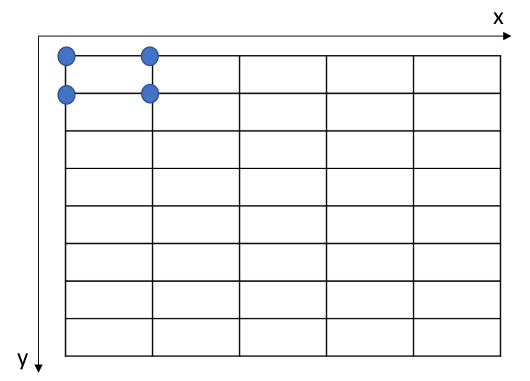
\includegraphics[width=2.5in]{figures/twoagent1.png}
  \caption{Arrangement of agents at the beginning(when $a=2$)}\label{fig:twoagent1}
\end{figure}

Let us now consider the routes for the agents, which will result to be a snake-like path. For convenience, we assume that all the agents move at time $t_i\,(i\in\mathbb{Z}^*)$  \color{blue} ??? because some time should be reserved for the coordination after the BV is triggered.??? In fact, we do not need to reserve time for the elimination. \color{black} 
%More detail about the moving cycle would be discussed after we decide the number of agents and the routes for them. 
Let $v=(x, y)$ be the node under exploration, with $1\leq x_i \leq d_1$, $1\leq y_i \leq d_2$. 
We define a boolean value called {\em Vertical Moving Mark}  (VMM) for every agent as follows: 
the value  VMM is initialized at zero and    every time   the agent moves SOUTH, it switches to  (VMM+1)mod 2. 
  For example, if an agent continues to move SOUTH  the VMM will keep alternating between 0 and 1, essentially indicating the parity of the row.
  
Every agent holds two VMMs in its memory  (say $VMM_1$ and $VMM_2$). 
The original value of $VMM_1$ is $0$; 
the original value of $VMM_2$ is 0 for the agents 
residing at node $(1, y)$ and  $1$ for the ones residing in node  $(2, y)$ ($1\leq y\leq a$).
We now define the action of the $2a$ agents:\\ 
\begin{itemize}
\item Let $b=a-1$. 
\color{blue} these should be local rules, how can the individual agent know that all values are zero. You have to express the rule in a different way, not replying on this type of info. (make some modification, please check)\color{black}

When an agent' s $VMM_1$ is ``0" and its $VMM_2$ is equal to ``0", then it moves EAST when $x\neq d_1-1$ and move SOUTH for $b$ steps when $x=d_1-1$;

When an agent' s $VMM_1$ is ``0" and its $VMM_2$ is equal to ``1", then it moves EAST when $x\neq d_1$ and move SOUTH for $b$ steps  when $x=d_1$;

When an agents' $VMM_1$ is ``1" and its $VMM_2$ is equal to ``0", then it moves WEST when $x\neq2$ and move SOUTH for $b$ steps when $x=2$;

When an agents' $VMM_1$ is ``1" and its $VMM_2$ is equal to ``1",  then it moves WEST when $x\neq 1$ and move SOUTH for $b$ steps when $x=1$.




\item An agent  moves only to a node that it has not explored yet. (Note that when residing at a node, an agent is able to know whether it has explored the neighbours of that node or not).
\end{itemize}

Informally, the resulting  routes of agents are snakelike routes. When $a=2$, the routes of agents are shown as Figure \ref{fig:twoagent2}. In order to show the routes more clearly, we present the routes of agents in different line respectively.
%\iffalse
\begin{figure} [H]
  \centering 
  \subfigure[Routes of agents in the first line when $a=2$]{ 
    \label{fig:agentroute:a} %% label for first subfigure 
    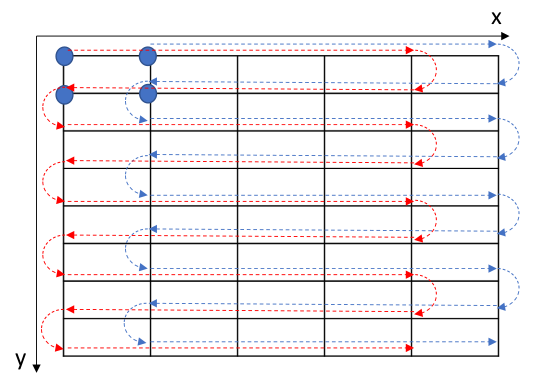
\includegraphics[width=3in]{figures/twoagentroute1.png}} 
 %\hspace{1in} 
  \subfigure[Routes of agents in the second line when $a=2$]{ 
    \label{fig:agentroute:b} %% label for second subfigure 
    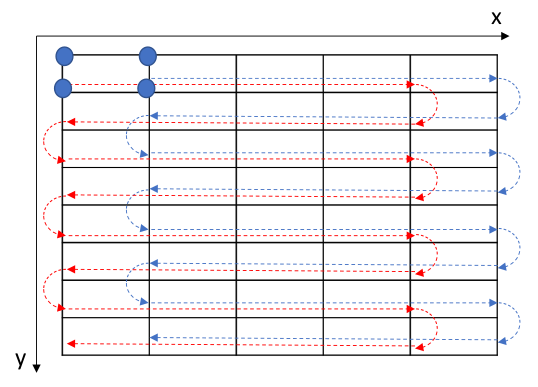
\includegraphics[width=3in]{figures/twoagentroute2.png}}
  \caption{Routes of agents when $a=2$} 
  \label{fig:twoagent2} %% label for entire figure 
\end{figure}
%\fi
 Figure \ref{fig:threeagent1} shows the routes of agents when $a=3$.
\begin{figure} [H]
  \centering 
  \subfigure[Routes of agents in the first line when $a=3$]{ 
    \label{fig:agentroute:a} %% label for first subfigure 
    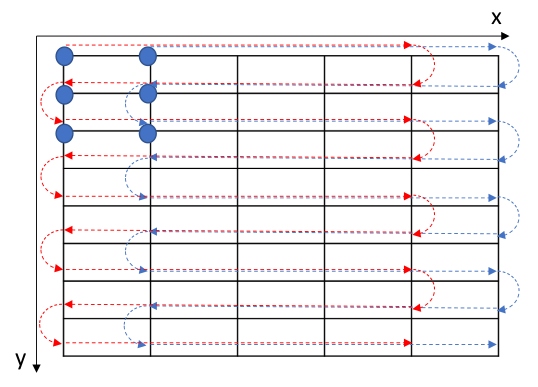
\includegraphics[width=3in]{figures/threeagentroute1.png}} 
  \hspace{1in} 
  \subfigure[Routes of agents in the second line when $a=3$]{ 
    \label{fig:agentroute:b} %% label for second subfigure 
    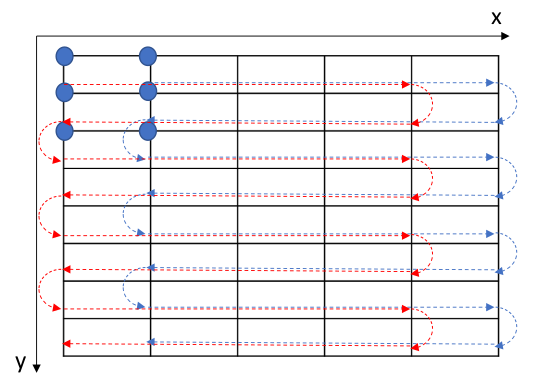
\includegraphics[width=3in]{figures/threeagentroute2.png}}
    \hspace{1in} 
    \subfigure[Routes of agents in the second line when $a=3$]{ 
    \label{fig:agentroute:c} %% label for second subfigure 
    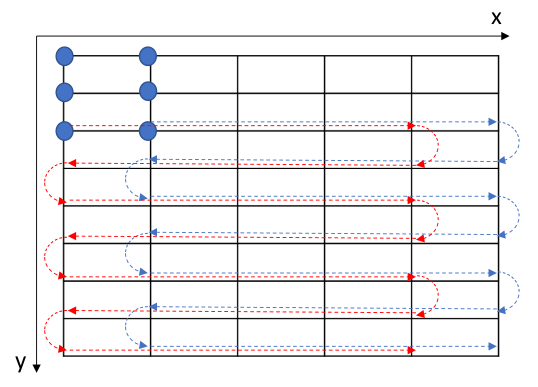
\includegraphics[width=3in]{figures/threeagentroute3.png}}
  \caption{Routes of agents when $a=3$} 
  \label{fig:threeagent1} %% label for entire figure 
\end{figure}

We can easily observe that some rows of the grid are traversed twice for the purpose of avoiding the explored nodes being contaminated (as shown in Fig \ref{fig:doubleline}).

\begin{figure} [H]
  \centering 
  \subfigure[Rows that are double traversed when $a=2$]{ 
    \label{fig:agentroute:a} %% label for second subfigure 
    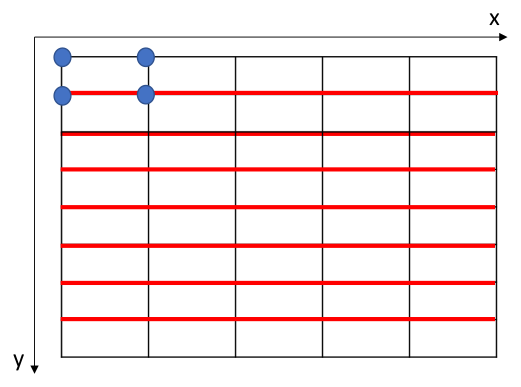
\includegraphics[width=3in]{figures/doubleline2.png}}
    %\hspace{1in} 
    \subfigure[Rows that are double traversed when $a=3$]{ 
    \label{fig:agentroute:b} %% label for second subfigure 
    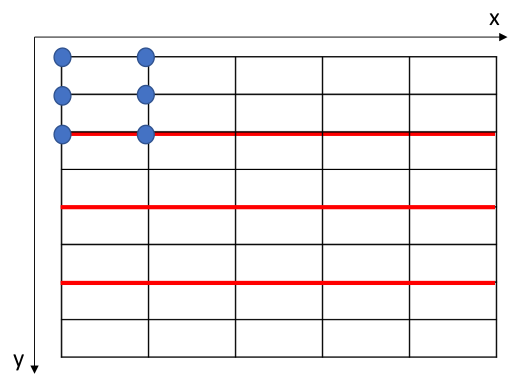
\includegraphics[width=3in]{figures/doubleline3.png}}
  \caption{Rows that are double traversed (marked with red rows)} 
  \label{fig:doubleline} %% label for entire figure 
\end{figure}

We can see that when the grid is fixed (so $d_1$ is fixed), the number of double traversed rows decrease as $a$ increases, which is easy to image. Let us denote by $r$ the number of rows that are double traversed, then $r=\left \lceil \frac{d_1-a}{a-1} \right \rceil$ where $d_1$ is the number of rows of the grid. Informally, $r$ indicates the time that is spent   in the exploration phase, and we can reduce this time by employing more agents. As we can see from the equation, when $a=d_1$, then $r=0$, which means if we employ $2d_1$ agents to explore the graph, none of the rows are traversed twice. \\
We now discuss the strategy when we employ $2d_1$ agents, and this strategy can be easily modified to fit the situation where we employ less than $2d_1$ agents.\\
Initially, 2$d_1$ agents are placed at the first two columns at $t_0$ and we place another  agent at the top and bottom of the first column (we shall describe their roles in the following part). More specifically, their coordinates   are (1, $x_i$) and (2,$x_i$) where $1\leq x_i\leq d_1$. The agents residing in the first column are in the shadowing group while the agents residing in the second column are in the exploring group. If the BV resides in a node of the first column, then all of its clones are destroyed. If the BV resides in a node in the second column, then the elimination phase begins. It is obvious that if the BV does not reside in any node in the first column, then an agent in the exploring group should be destroyed when the BV is exposed.  Let us assume that the we starts at $t_0$. Agents residing in nodes of the second column move  EAST at the beginning of $t_i$, $i=0,1, \ldots ,d_2-1$. More precisely, the agent located in $(x, y)$ moves to $(x+1, y)$ at the beginning of $t_i$, $i=0,1, \dots , d_2-1$. Agents residing in the first column simply follow the node in the second column (see  Fig.\ref{fig:moving}). When one of the nodes in the second  column is destroyed by a BV, the second phase starts.
\begin{figure}[H]
  \centering  
  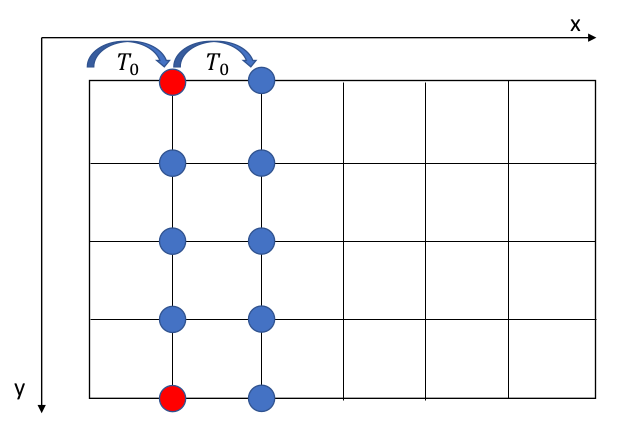
\includegraphics[width=2.5in]{figures/moving.png}
  \caption{Agents move at time $t_0$. (The red node indicates that there are two agents residing there}\label{fig:moving}
\end{figure}
\noindent{\bf Elimination Phase}\\
The elimination begins when one of the nodes in the second column is destroyed by a BV (let us say, at time $t_i$). No matter where   the BV is, there are always three agents residing on its north (if the BV is not in the first row), west and south (if the BV is not in the last row), so only one BV clone survives. In another words, only one node becomes BV   after the BV has been triggered. Observe that in the parallel strategy, not all agents participate in the elimination phase automatically when the BV is explored because only the ones  that receive the clones of the original BV and those that are notified by other agents can participate in the elimination phase. So,  in some situations, agents that receive the BV clone should notify other agents to participate in the elimination (cases 1,2 and 3 below). In one particular situation (case 4 below), we  instead use the agent  that we take along the way (called  following agent) to complete the elimination phase. Let the node where the surviving clone reside be $(x, y)$. We have four different situations   depending on the location of the new formed BV, each situation corresponding to a different route  taken in the elimination phase.
\begin{itemize}
\item Case 1: When $2<x<d_1$, $1<y<d_2-1$ (an interior node becomes a new formed BV), then the agents residing in node $(x-1, y+1)$, $(x-1, y-1)$ and $(x-2, y)$ (say $a,b,c$) receive a BV clone at time $t_i$, and  they know the location of the original BV and also the new formed BVs. After they receive the BV clone, these agents move EAST at $t_{i+1}$ for one step (for example, to node $(x, y+1)$, $(x, y-1)$ and $(x-1, y)$) and stop. Note that other agents including the ones residing in node $(x-2, y+1)$ and $(x-2, y-1)$ (say agent $d$ and $e$) at $t_i$ do not know the existence of the BV so they keep moving EAST and arrive at nodes $(x, y+1)$, $(x, y-1)$ at the end of $t_{i+2}$ when they meet agent $a$ and $b$ respectively. Agent $a$ and $b$ inform them of the location of the new formed BV and the routes of agents $d$ and $e$ are as follow:\\
route of $d$: $(x, y+1)(at\ t_{i+2}){\rightarrow}(x+1,y+1)(at\ t_{i+3}){\rightarrow}(x+1,y)(at\ t_{i+4})$.\\
route of $e$: $(x, y-1)(at\ t_{i+2}){\rightarrow}(x, y)(at\ t_{i+5})$.

The routes of agents are showed in Fig.\ref{fig:caseone} where ``one circle" indicates that there is one agent residing here; ``two circle" indicates that there are two agents residing here; ``three circle" indicates that there are three agents residing here. 

%\iffalse
\begin{figure} [H]
  \centering 
  \subfigure[$t_i$]{ 
    \label{fig:caseone0:a} %% label for first subfigure 
    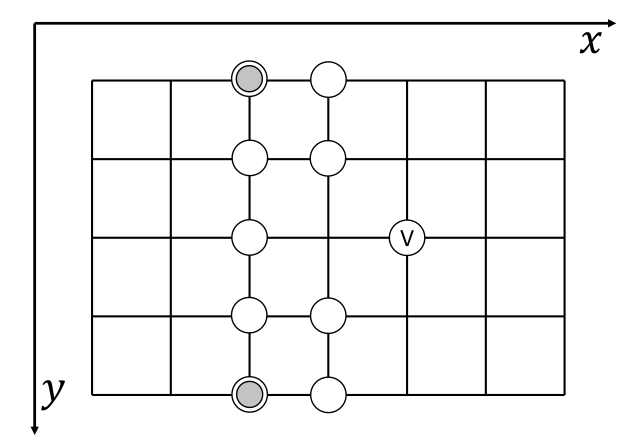
\includegraphics[width=2.5in]{figures/caseone0.png}} 
%  \hspace{1in} 
  \subfigure[$t_{i+1}$]{ 
    \label{fig:caseone1:b} %% label for second subfigure 
    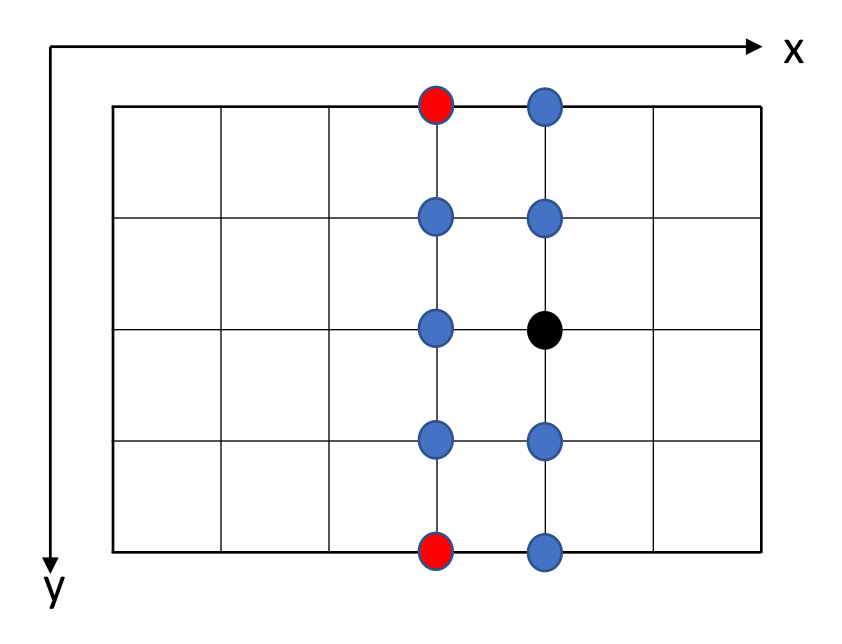
\includegraphics[width=2.5in]{figures/caseone1.png}}
    \hspace{1in} 
  \subfigure[$t_{i+2}$]{ 
    \label{fig:caseone2:c} %% label for second subfigure 
    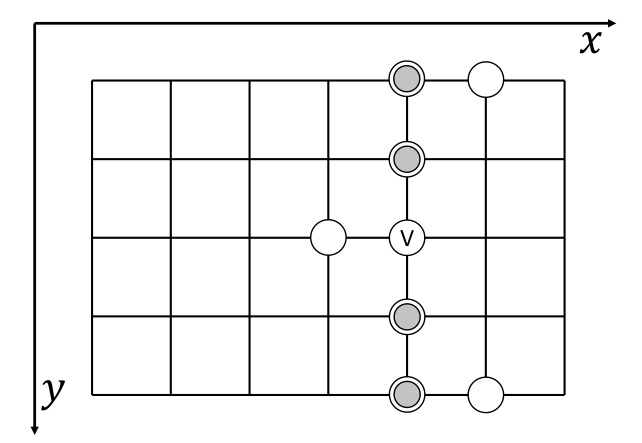
\includegraphics[width=2.5in]{figures/caseone2.png}}
%      \hspace{1in} 
  \subfigure[$t_{i+3}$]{ 
    \label{fig:caseone3:d} %% label for second subfigure 
    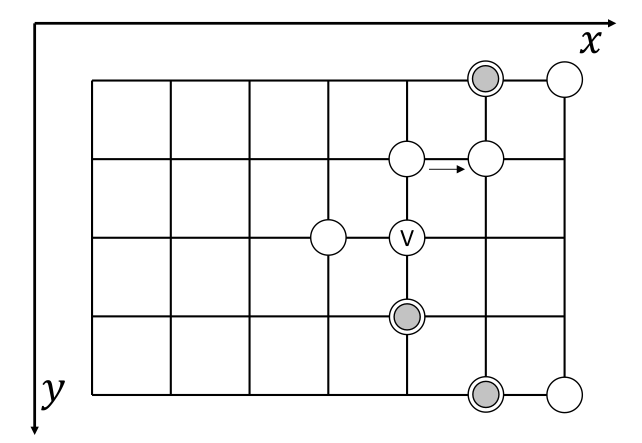
\includegraphics[width=2.5in]{figures/caseone3.png}}
      \hspace{1in} 
  \subfigure[$t_{i+4}$]{ 
    \label{fig:caseone4:e} %% label for second subfigure 
    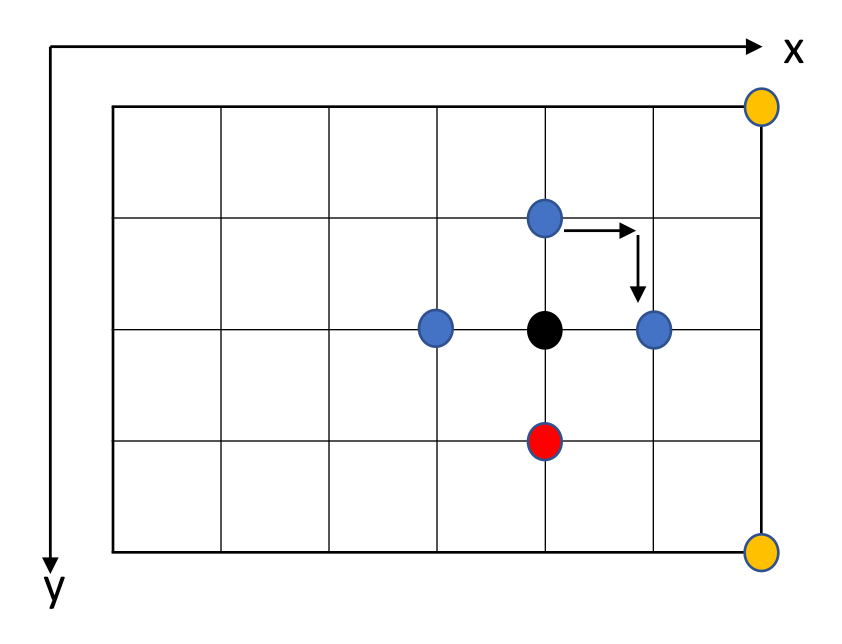
\includegraphics[width=2.5in]{figures/caseone4.png}}
     \subfigure[$t_{i+5}$]{ 
    \label{fig:caseone5:e} %% label for second subfigure 
    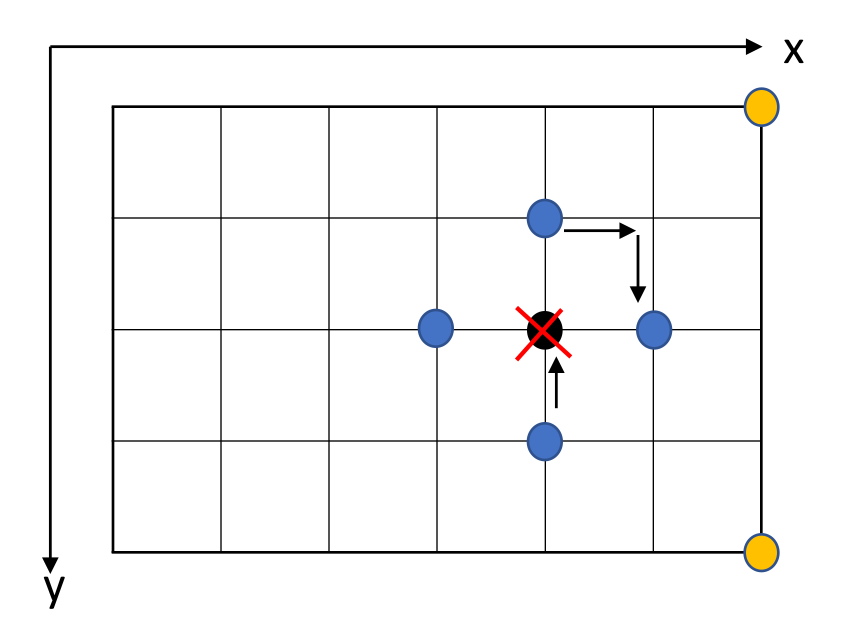
\includegraphics[width=2.5in]{figures/caseone5.png}}
  \caption{Arrangement of the agents in elimination phase when the new formed BV resides in a interior node} 
  \label{fig:caseone} %% label for entire figure 
\end{figure}
%\fi

\item Case 2: When $x=d_1$, $2<y<d_2-1$ (a border node becomes a new formed BV), then the agents residing in node $(x-1, y+1)$, $(x-1, y-1)$ and $(x-2, y)$  (say  $a,b,c$)  receive a BV clone at time $t_i$. As above, they move EAST for one step and stop. The agents residing in nodes $(x-2, y+1)$ and $(x-2, y-1)$ (say  $a,b$) at $t_i$ have no knowledge of the BV, so they keep moving and arrive at nodes $(x, y+1)$ and $(x, y-1)$ at $t_{i+2}$ when they are informed of the location of the new formed BV. 
One of the agents  should move to the new formed BV to decontaminate it while the other stops moving at $t_{i+3}$. In order to avoid conflict, we always employ the agent  who observes that the BV is in its SOUTH (say agent $a$) to move to the new formed BV  (see Fig \ref{fig:casetwo}).
\begin{figure} [H]
  \centering 
  \subfigure[$t_i$]{ 
    \label{fig:casetwo0:a} %% label for first subfigure 
    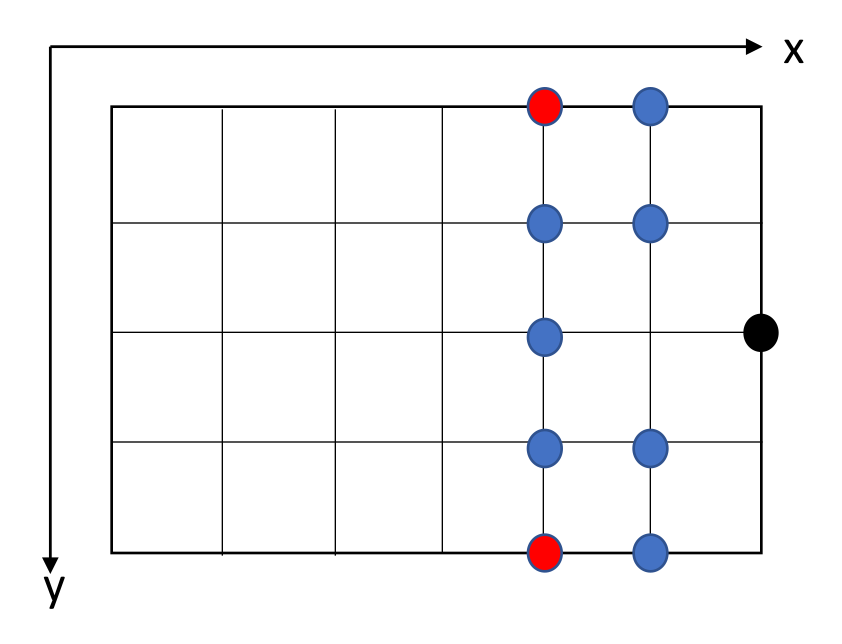
\includegraphics[width=2.5in]{figures/casetwo0.png}} 
%  \hspace{1in} 
  \subfigure[$t_{i+1}$]{ 
    \label{fig:casetwo1:b} %% label for second subfigure 
    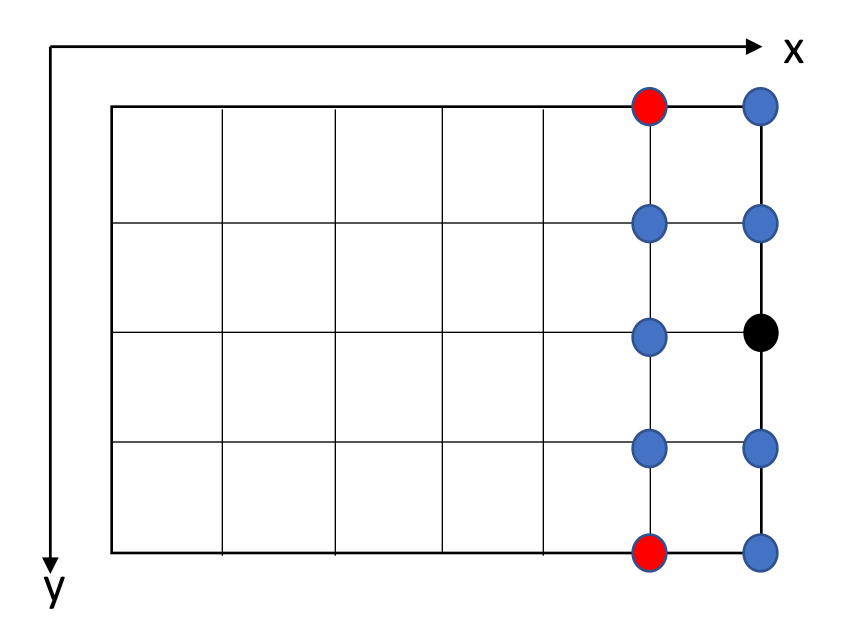
\includegraphics[width=2.5in]{figures/casetwo1.png}}
    \hspace{1in} 
  \subfigure[$t_{i+2}$]{ 
    \label{fig:casetwo2:c} %% label for second subfigure 
    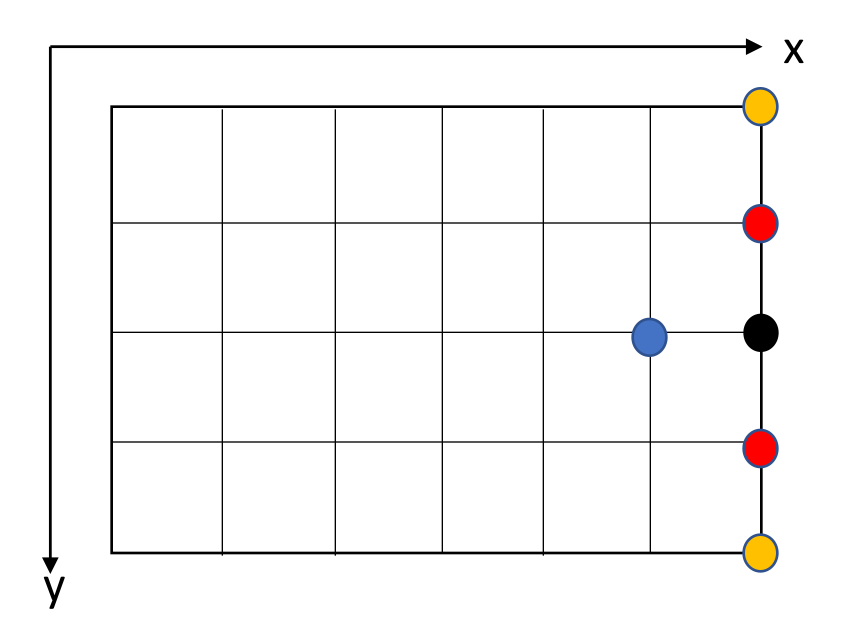
\includegraphics[width=2.5in]{figures/casetwo2.png}}
%      \hspace{1in} 
\subfigure[$t_{i+3}$]{ 
    \label{fig:casetwo3:d} %% label for second subfigure 
    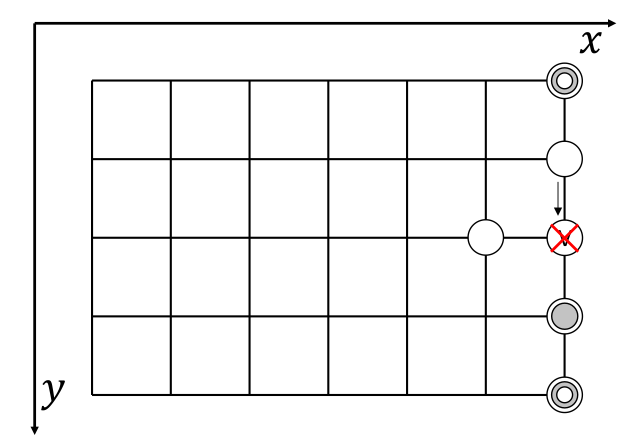
\includegraphics[width=2.5in]{figures/casetwo3.png}}
    \caption{Arrangement of the agents in the elimination phase when the new formed BV resides in a border node (when $x=d_1$)} 
  \label{fig:casetwo} %% label for entire figure 
\end{figure}

\item Case 3: When $2<x<d_1$, $y=1$ or $y=d_2-1$ (a border node becomes a new formed BV). For convenience, we only discuss the situation when $y=1$(the solution can be easily modified to fit the scenario when $y=d_2-1$). In this case, agents residing in nodes $(x-1, y+1)$ and $(x-2, y)$ (say  $a,b,c$, where $c$ is the following agent) receive a BV clone at time $t_i$. Agents $a$, $b$ and $c$ move EAST for one step and arrive at node $(x, y+1)$ and node $(x-1, y)$ at $t_{i+1}$. The agent in node $(x-2, y+1)$ (say, $d$) does not know the existence of the BV, so it keeps moving arriving at node $(x, y+1)$ at $t_i+2$. After that, the routes of the agents $c$ (the following agent) and $d$ are described  below:\\
route of $d$: $(x, y+1)(at\ t_{i+2}{\rightarrow}(x+1,y+1)(at\ t_{i+3}{\rightarrow}(x+1,y)(at\ t_{i+4})$.\\
route of $c$: $(x-1, y)(at\ t_{i+2}{\rightarrow}(x, y)(at\ t_{i+5})$.


%\iffalse
\begin{figure} [H]
  \centering 
  \subfigure[$t_i$]{ 
    \label{fig:casethree0:a} %% label for first subfigure 
    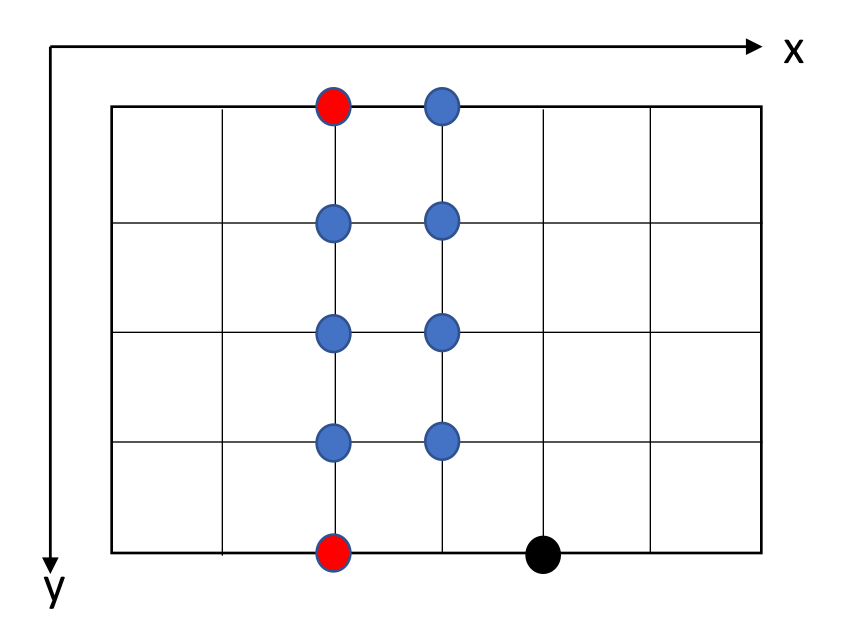
\includegraphics[width=2.5in]{figures/casethree0.png}} 
%  \hspace{1in} 
  \subfigure[$t_i+1$]{ 
    \label{fig:casethree1:b} %% label for second subfigure 
    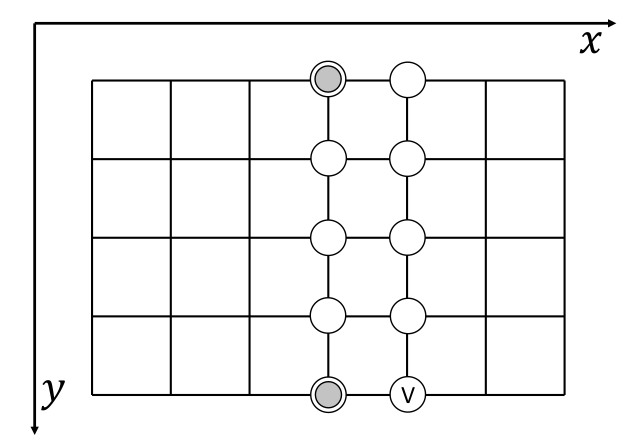
\includegraphics[width=2.5in]{figures/casethree1.png}}
    \hspace{1in} 
  \subfigure[$t_{i+2}$]{ 
    \label{fig:casethree2:c} %% label for second subfigure 
    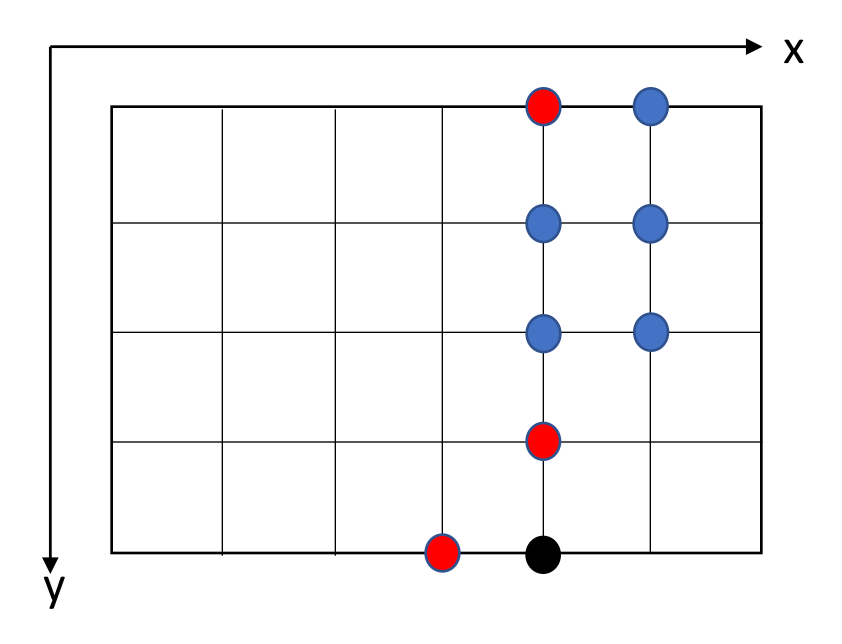
\includegraphics[width=2.5in]{figures/casethree2.png}}
%      \hspace{1in} 
  \subfigure[$t_{i+3}$]{ 
    \label{fig:casethree3:d} %% label for second subfigure 
    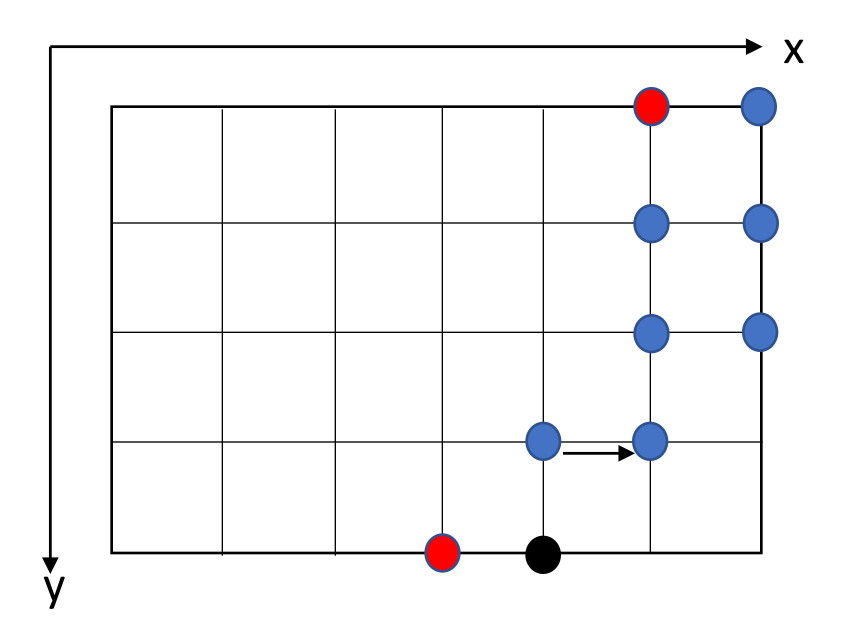
\includegraphics[width=2.5in]{figures/casethree3.png}}
      \hspace{1in} 
  \subfigure[$t_{i+4}$]{ 
    \label{fig:casethree4:e} %% label for second subfigure 
    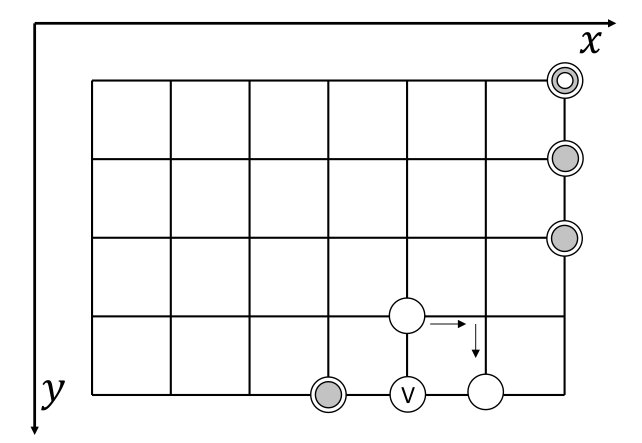
\includegraphics[width=2.5in]{figures/casethree4.png}}
     \subfigure[$t_{i+5}$]{ 
    \label{fig:casethree5:e} %% label for second subfigure 
    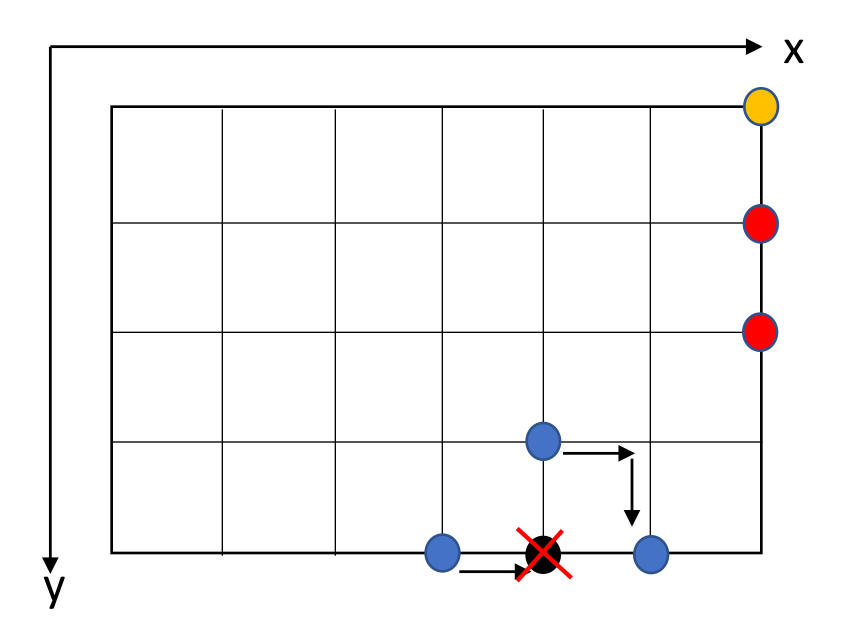
\includegraphics[width=2.5in]{figures/casethree5.png}}
  \caption{Arrangement of the agents in the  elimination phase when the new formed BV resides in a border node(when $y=1$ or $y=d_2-1$)} 
  \label{fig:casethree} %% label for entire figure 
\end{figure}
%\fi

\item Case 4: When $x=d_1$ and $y=1$ or $y=d_2-1$ (a corner node becomes a new formed BV). For convenience, we only discuss the situation when $y=1$ and with some simple modification, the strategy can fit the scenario when $y=d_2-1$.  In this case, agents residing in node $(x-1, y+1)$ and $(x-2, y)$ (say, $a,b$) receive a BV clone at $t_i$. Both of them keep moving for one step arriving  at nodes $(x, y+1)$ and $(x-1, y)$ at $t_{i+1}$. Then agent $b$ moves to the BV to destroy it at $t_{i+2}$
\begin{figure} [H]
  \centering 
  \subfigure[$t_i$]{ 
    \label{fig:casefour0:a} %% label for first subfigure 
    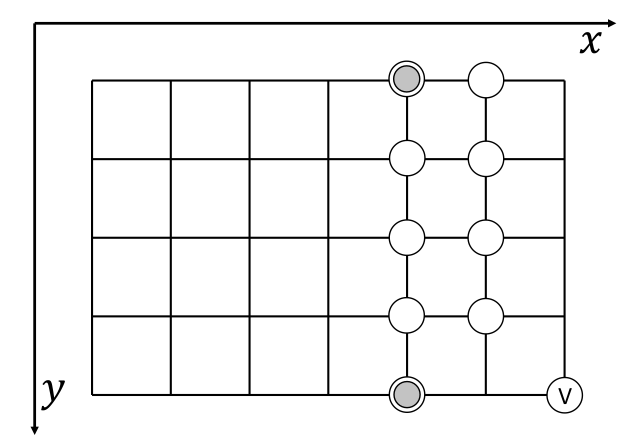
\includegraphics[width=2.5in]{figures/casefour0.png}} 
% \hspace{1in} 
  \subfigure[$t_{i+1}$]{ 
    \label{fig:casefour1:b} %% label for second subfigure 
    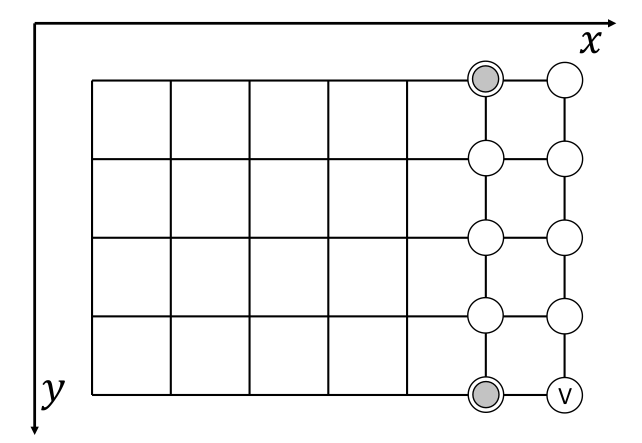
\includegraphics[width=2.5in]{figures/casefour1.png}}
 \hspace{1in} 
  \subfigure[$t_{i+2}$]{ 
    \label{fig:casefour3:c} %% label for second subfigure 
    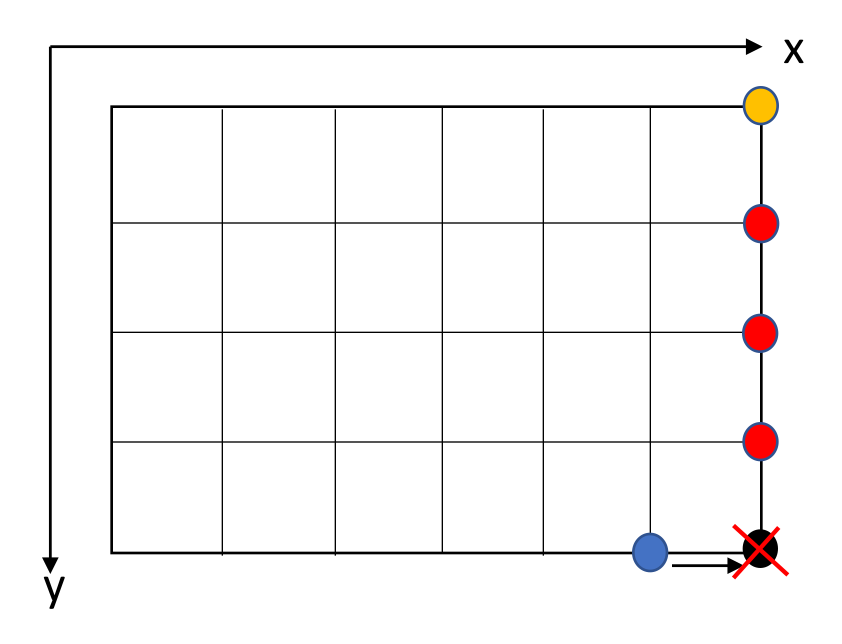
\includegraphics[width=2.5in]{figures/casefour3.png}}
%      \hspace{1in} 
%\subfigure[$T(t_i+3)$]{ 
   % \label{fig:casefour3:d} %% label for second subfigure 
    %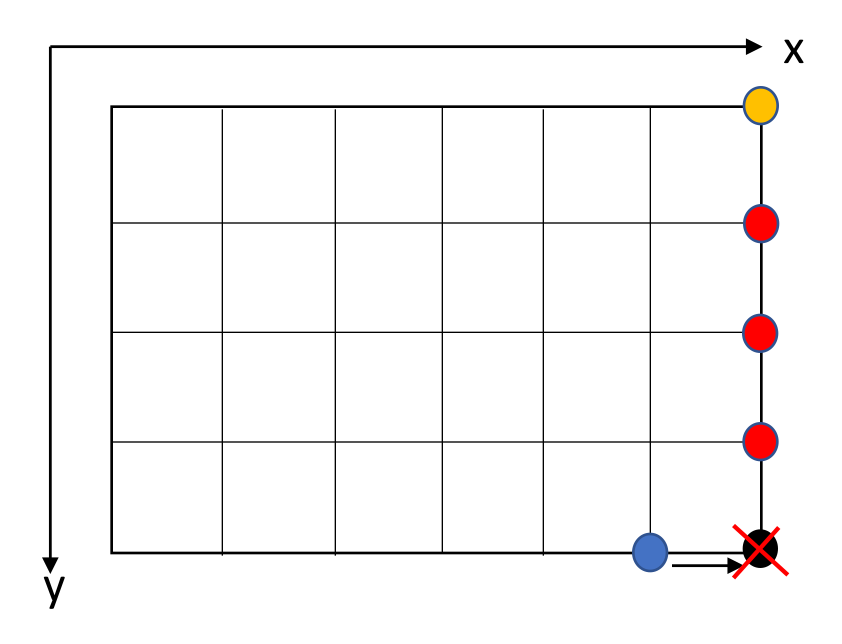
\includegraphics[width=2.5in]{figures/casefour3.png}}
    \caption{Arrangement of the agents in the elimination phase when the new formed BV resides in a corner node(when $x=d_1$ and $y=1$ or $y=d_2-1$)} 
  \label{fig:casefour} %% label for entire figure 
\end{figure}
\end{itemize}

\noindent{\bf Analysis and Comparisons}

Let ${\cal M}$ be a mesh of size   $n=d_1\times d_2$  with $d_1=min\{d_1, d_2)\}$.
 
\begin{theorem}
Algorithm $PBVD-2G$  performs a decontamination of  ${\cal M}$  
 using $k=2(d_1+1)$  agents (that is, $(2(\sqrt{n}+1)$ agents   in the worst case),
 and incurring in at most 1 casualty. 
\end{theorem}
\begin{proof}
Let $v=(x, y)$ be the node containing the BV. When one of the agents in the exploring group moves to $v$, it will be destroyed and the BV will move to all neighbours of $v$. If $x=1$, then the neighbours $(x, y+1)$, $(x, y-1)$ and $(x+1, y)$ are protected by agents and neighbour $(x-1, y)$ actually does not exist; if $x>1$, then neighbours $(x, y+1)$, $(x, y-1)$ and $(x-1, y)$ are protected by agents. So when the clones of BV moves to the neighbours of $v$, the nodes that contain an agent will not be infected by the BV clone; this means that the BV can safely move only to the unexplored neighbours of $v$,   which is at most one. In other words, after $v$ is explored, at most one BV node is formed. According to our elimination strategy, the new formed BV node can be surrounded and destroyed using at most five agents: one to enter a BV and four to protect the neighbours. Since we have one new formed BV, the number of agents participating in the elimination phase is at most five. In addition to the agent destroyed by the original BV, the number of agent needed to complete the elimination phase is at least six. Since we employ $k=2d_1+2$ ($d_1\geq 3$) which means at the beginning we have at least eight agents, so $2d_1+2$ agents are enough for the decontamination algorithm. In the worst case (which is the case of a  square mesh where $d_1=d_2$) the number of agent is equal to $2\sqrt{n}+2$.
\end{proof}
Let us now consider the number of movements.
\begin{theorem}
Algorithm $PBVD-2G$  performs a BV decontamination  of ${\cal M}$ with at most $2n-\sqrt{n}+O(1)$ movements and at most $\sqrt{n}+11$ in time.
\end{theorem}
\begin{proof}
Let $v=(x, y)$ be the BV node, and let the size of the grid be $n=d_1\times d_2$. Let us first consider the number of movements performed during the shadowed exploration. Since all the agents simply move EAST at the beginning of $T(2n)$ ($n=0,1, \dots , d_2-1$), the travelling distance is $x$ for agents in the exploring group ({\em EA}) and $x-1$ for agents in the shadowing group ({\em SA}). We   have $d_1$ {\em EAs} and $d_1+2$ {\em SAs}, then we have an overall cost of at most $2x(d_1+1)-(d_1+2)$ movements for this phase.
Consider now the number of movements performed for Surrounding and Elimination. In this part, we only compute the movements of the agents that participate in the Surrounding and Elimination. More specifically, we   ignore the movements of the agents that do not know the existence of the BV in the whole process. As we discussed in the Elimination phase, when the new formed BV is located in an interior node, eight movements are needed in this phase; when the newly formed BV is located in a border node (say $(a, b)$), then six movements are needed when $a=d_1, 2< b <d_2-1$ and eight movements are needed when $2< a <d_1,b=1\,or\,b=d_2-1$; when the newly formed BV is located in a corner node, then four movements are needed in this phase. Hence, $O(1)$ movements are performed in this phase.
In total we have that the number of movements is at most $2x(d_1+1)-(d_1+2)+O(1)\leq 2\sqrt{n}( \sqrt{n}+1)-(\sqrt{n}+2)+O(1)$, which is $2n+\sqrt{n}+O(1)$.\\
As for the time complexity. The time required for the exploration phase is equal to the number of movements of each EA, which is $d_1$; the time required for the surrounding and elimination phase is at most eleven. So in total the parallel mesh decontamination algorithm terminate in time at most $\sqrt{n}+11$. 
\end{proof}

Table \ref{table:ComparisionPBVD-2GandBVD-2G}  shows a comparison between our strategy and the sequential strategy.

\begin{table} [hbtp]
\caption{Comparison between PBVD-2G and BVD-2G}
\label{table:ComparisionPBVD-2GandBVD-2G}
\centering
\tabulinesep=2mm
\begin{tabu} to 140 mm {|X[6,c]|X[4,l]|X[4,l]|X[4,l]|X[4,l]|} \hline 
%\begin{tabular}{|c|l|} \hline 
&   agents &   time   &   movements &   casualties \\ \hline
{\em PBVD-2G}   &$2(d_1+1)$ $(d_1=min(d_1, d_2))$& $\sqrt{n}+11$   & $2n+\sqrt{n}+O(1)$   & 1        \\ \hline
{\em BVD-2G} & 7    & $3n$          & $9n+O(1)$     & 3              \\ \hline
\end{tabu}
%\end{tabular}
\end{table}


\subsection{Multi-Dimensional Grid}
Let $M$ be a q-dimensional grid of size $d_1\times\ldots\times d_q$ and let each node of $M$ be denoted by its coordinates $(x_1,\ldots,x_q)$, $1\leq x_i\leq d_q$. The algorithm, called {\em PBVD-qG}, follows a general strategy similar to the one described in Section 4.2.1: a safe exploration with shadowing, followed by a surrounding and elimination phase. Our general idea is as follows: (1) Transform the PBVD-qG problem into a BVD-qG problem (2) Use the BVD-qG strategy to solve the transformed problem.

 %
In \cite{cai}, the multi-dimensional grid is partitioned into $d_1\times \ldots d_{q-2}$ 2-dimensional grids of size $d_{q-1} \times d_q$. Each of these grids is explored using the BVD-2G: after traversing a grid in a snake-like fashion column by column, the agent returns to the starting point and from that starting point, it proceeds to another grid with a neighbouring starting point. In our strategy PBVD-qG, we use the similar exploring routes as that in BVD-G, which is the snake-like route. Additionally, we use the idea of {\em dimensionality reduction}.
In our  parallel strategy   we use the term  ``p-dimensional  agent group" to 
refer to a group of $d_1\times \ldots \times d_p$ agents   ($p<q$) organized in a $d_1\times \ldots \times d_p$ grid (i.e.,   fully occupying  a $d_1\times \ldots \times d_p$ sub-grid of the original $q$-dimensional grid). 
Informally, a ``p-dimensional  agent group" 
can  be viewed as one  ``large agent" and  the  q-dimensional grid as a  ``virtual"  $(q-p)$-dimensional grid.
Clearly, the larger $p$, the smaller the size of the virtual grid to be explored (see Figure \ref{fig:4dimensional} for examples). 
%
%  So, when we increase the number of the agents (i.e.,  increase   ``p" in the group), then   we implicitly  decrease the dimension of the grid we want to explore. For example, if we want to solve the BVD problem in a 4-dimensional grid (say in a $d_1\times\ d_2 \times d_3\times d_4$ grid) using the PBVD-2G and we use $d_1$ agents to explore it. The problem can be viewed as using one ``large" agent to explore a $d_2\times d_3\times d_4$ grid. If we use $d_1\times d_2$ agents to explore it, then the problem can be viewed as using one ``large" agent to explore a $d_3 \times d_4$ grid. We can choose the dimension of the agent group at the beginning, and Figure \ref{fig:4dimensional} shows how can we view a higher dimensional grid as a lower dimensional grid. 

\begin{figure} [H]
  \centering 
  \subfigure[The arrangement of agents on a 4-dimensional grid]{ 
    \label{fig:4dimensional1:a} %% label for first subfigure 
    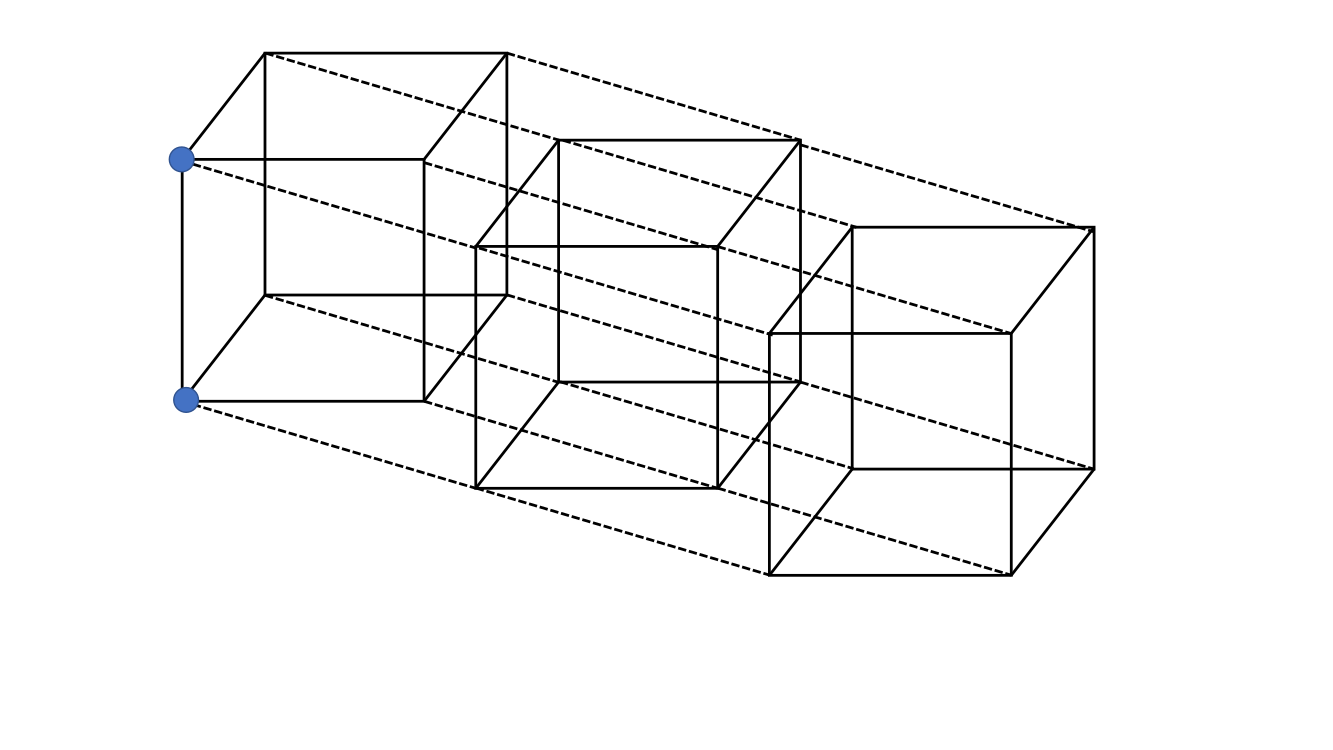
\includegraphics[width=2.8in]{figures/4dimensional1.png}} 
% \hspace{1in} 
  \subfigure[When we view the ``one dimensional" agent as a large agent and the grid can be view as a three dimensional grid]{ 
    \label{fig:4dimensional2:b} %% label for second subfigure 
    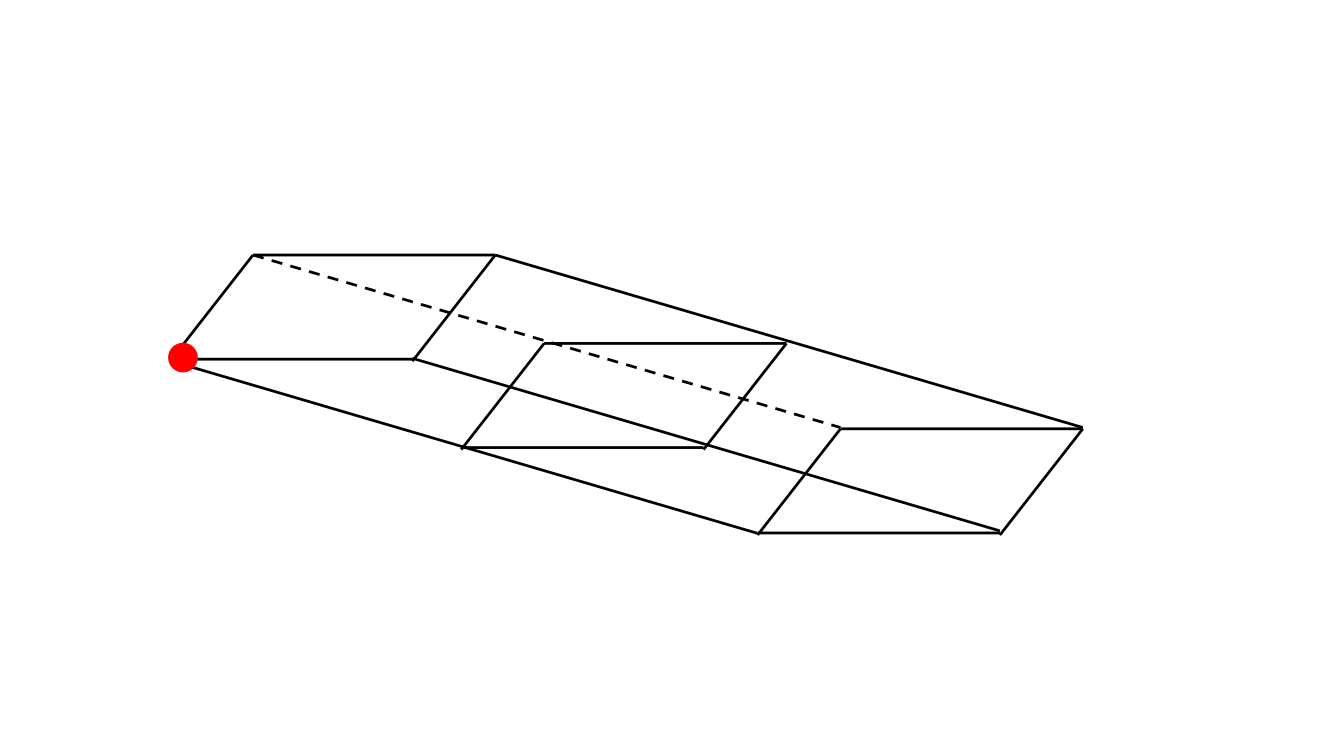
\includegraphics[width=2.8in]{figures/4dimensional2.png}}
 \hspace{1in} 
  \subfigure[The arrangement of agents on a 4-dimensional grid]{ 
    \label{fig:4dimensional3:c} %% label for second subfigure 
    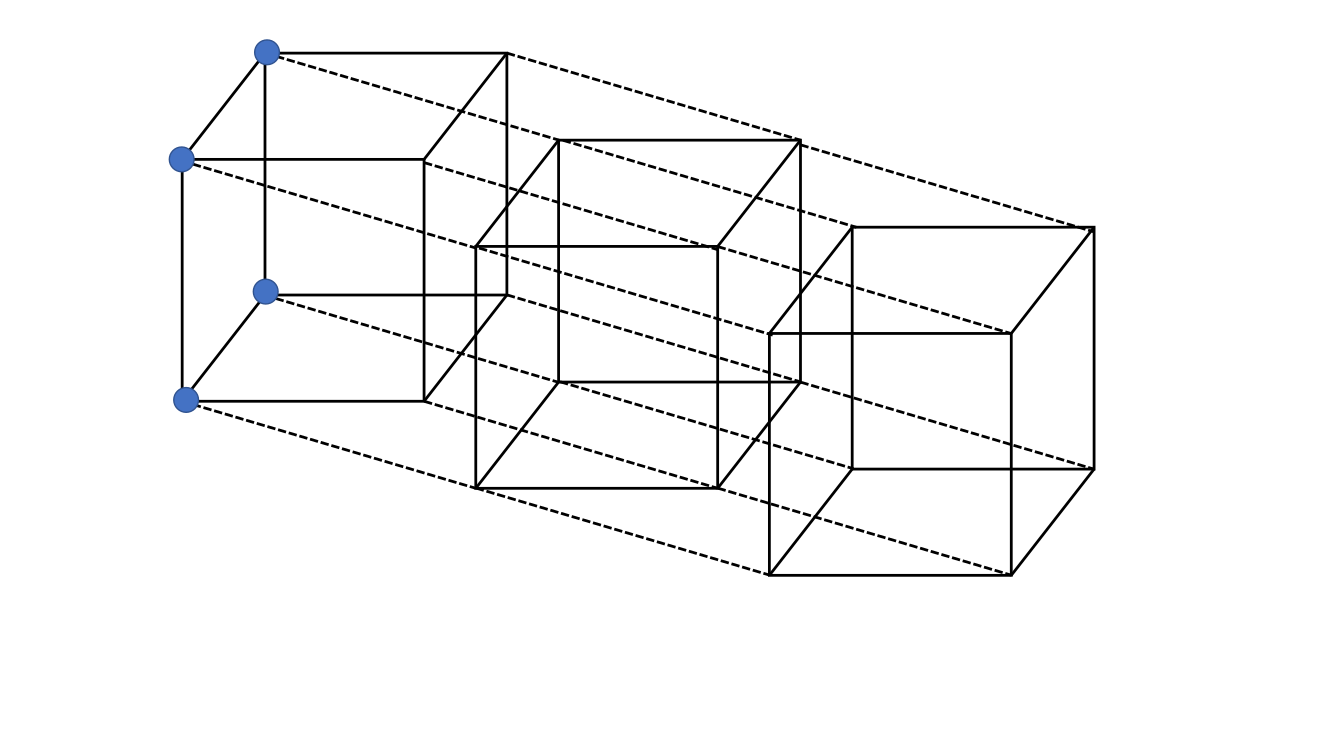
\includegraphics[width=2.8in]{figures/4dimensional3.png}}
%\hspace{1in} 
\subfigure[When we view the ``two dimensional" agent as a large agent and the grid can be view as a two dimensional grid]{ 
    \label{fig:4dimensional4:d} %% label for second subfigure 
    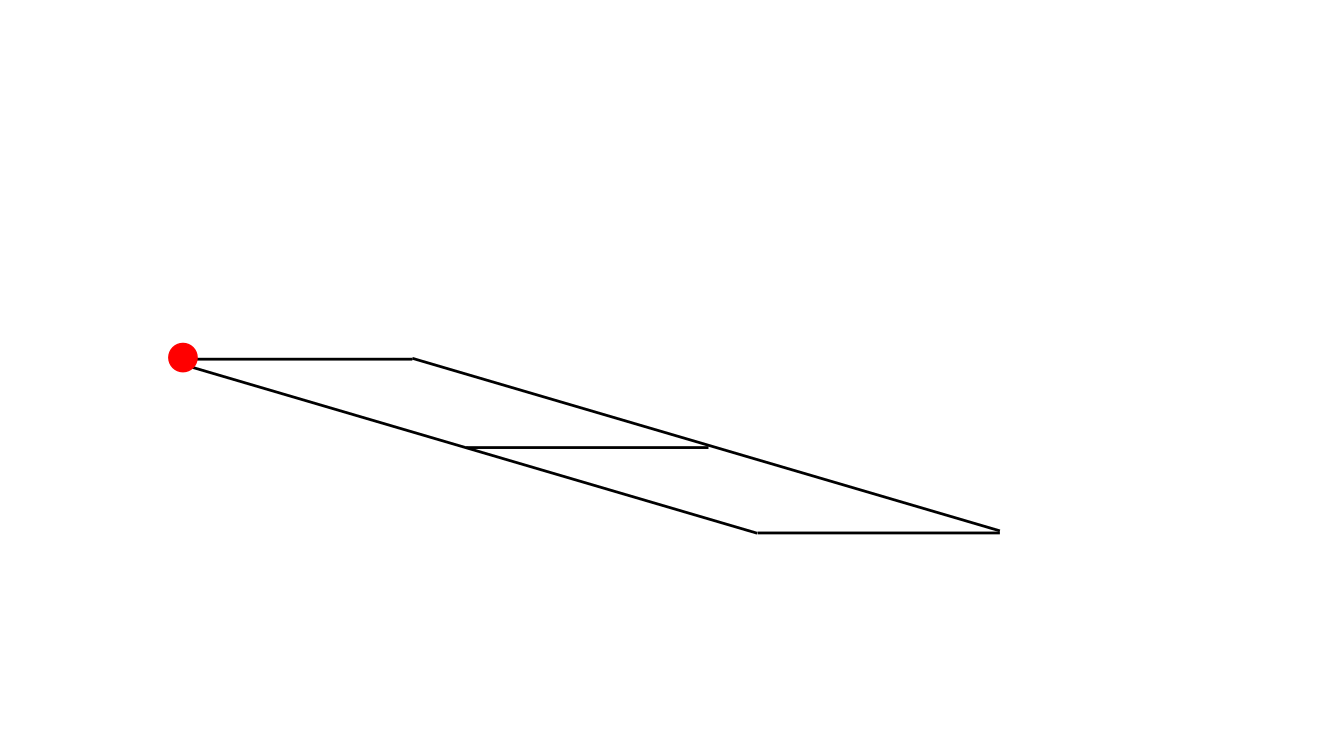
\includegraphics[width=2.8in]{figures/4dimensional4.png}}
    \caption{The idea of dimensionality reduction} 
  \label{fig:4dimensional} %% label for entire figure 
\end{figure}
After we transform the problem,   we can use the BVD-qG to solve the PBVD-qG. 
Let us  now have a brief review of the  BVD-qG strategy:  there are two agents exploring the graph: one is called exploring agent (EA) and one is called leader exploring agent (LEA). They follow the ``four step cautious walk" strategy  to explore the graph: before exploring a node $v=(x_1, \ldots, x_q) (1\leq x_i \leq d_i)$ from a node $u$, the shadowing agents(SA) move to the already explored neighbours of $v$ (whose coordinated can be precisely computed). When EA visits the BV node (and is destroyed there), the LEA and the SAs are aware of the location of the new BV nodes  (its coordinates  can be   computed precisely).
 So, once the node  $v$ containing the BV is identified, $2q$ agents surround each node $u\in N_{un}(v)$ and an additional agent enters it destroying the BV resident there and the instances that it generates. 
 
 %Note that in \cite{Cai},   protocol BVD-qG use $3q+1$ agents;  by viewing the  $d_1\times\ldots d_p$ agents as a ``big agent" then applying the BVD-qG protocol,   we need in total  $d_1\times \ldots d_p\times (3q+1)$ agents. {\bf (doesn't this contradicts the theorem below ? In any case, to be moved later})

%We have map the $``d_1 \times \ldots \times d_p" (1\leq p\leq q)$ agents into one ``big agent". 

Assume that we employ a ``p dimensional" agent group, which consists of $d_1 \times \ldots d_q$ agents with coordinates: $(x_1, \ldots, x_p, \ldots, x_q)$, $(1\leq x_1\leq d_1, \ldots, 1\leq x_p\leq d_p, x_{p+1}=0, \ldots, x_q=0)$. Then the coordinates of the ``big agent" in the $q-p$ dimensional grid are  $(x_{p+1},\ldots, x_q)$.
The first $p$ dimensional coordinates of the agents would not change in the whole exploring phase, but from that $(p+1)^{th}$ dimensional coordinates, they  change as the ``big agent" changes. More specifically, the coordinates of the  $(p+1)^{th}$ dimension   of the agents make the same change as the first dimensional coordinate of the ``big agent"; the coordinates of the  $(p+2)^{th}$  dimension of the agents make the same change as the second dimensional coordinate of the ``big agent", and so on. 
Assume  now that we   employ four agents (two agents are viewed as the LEA in the BVD-qG; two agents are viewed as the EA in the BVD-qG) to explore the 4-dimensional grid (they traverse the grid with the same routes following ``four step cautious walk"), then the routes of the agents are as below (see Fig.\ref{fig:grouproute}):
\begin{figure} [H]
  \centering 
  \subfigure[The route of the ``big agent"(LEA in the BVD-qG)]{ 
    \label{fig:grouproute1:a} %% label for second subfigure 
    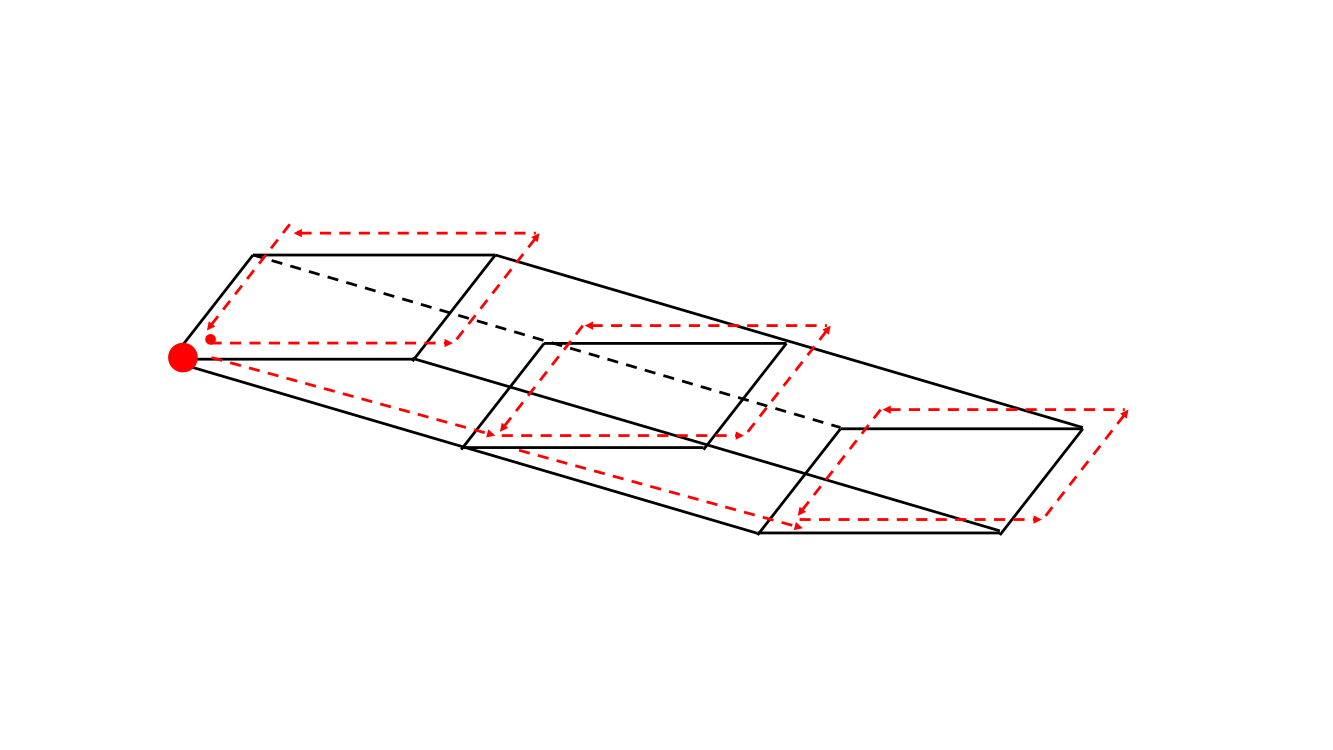
\includegraphics[width=3.5in]{figures/grouproute1.png}}
    \hspace{1in} 
\subfigure[The routes of the 2 agents viewed as the ``big agent"]{ 
    \label{fig:grouproute2:d} %% label for second subfigure 
    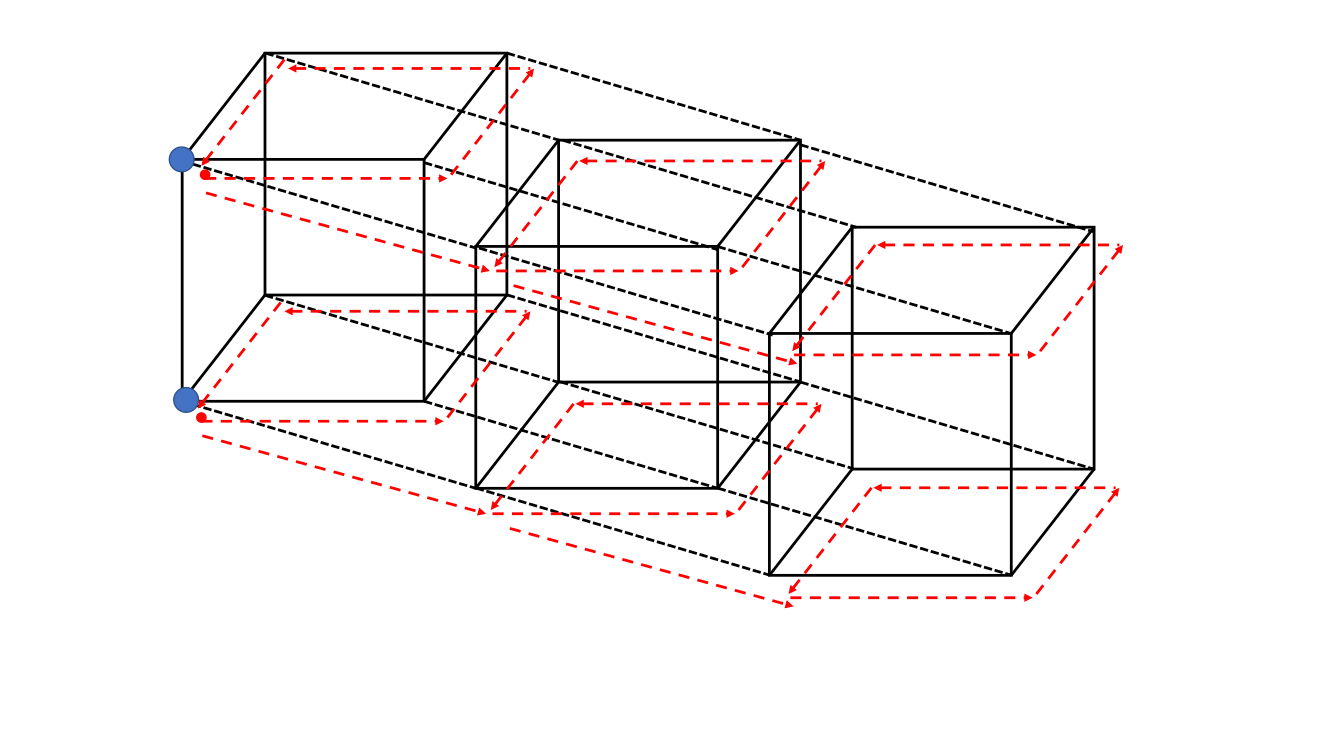
\includegraphics[width=3.5in]{figures/grouproute2.png}}
    \caption{The route of agent when exploring a $1\times1\times1\times2$ grid } 
  \label{fig:grouproute} %% label for entire figure 
\end{figure}

\noindent{\bf Analysis and Comparisons}
We now compare the time cost, the number of movements and the casualties with different number of agents we employ (Assuming that we are in a $d_1\times \ldots \times d_q$ q-dimensional grid).
The theorems in \cite{cai} show   that the protocol BVD-qG performs a BV decontamination of a q-dimensional Grid using $3q+1$ agents with at most $q+1$ casualties and  at most $O(qn)$ movements and $\Theta(n)$ time. Based on these theorems, we now discuss the number of agents, the casualties, the time cost and the number of movement in PBVD-qG.

 Let ${\cal M}_q$ be a   q-dimensional grid of size   $n=d_1  \times  \ldots \times  d_p \times  \ldots   \times  d_q $.
 \color{black}
 
\begin{theorem}
PBVD-qG performs a decontamination of  ${\cal M}_q$ using $2\times d_1\times \ldots d_p (1\leq p\leq q)$ 
agents and at most $q-p+1$casualties, with at most $O(qn)$ moves  and $\Theta(\frac{n}{d_1\times\ldots\times d_p})$ time.
\end{theorem}

\begin{proof}
In PBVD-qG, we can choose different number of agents to start the exploration, and that number results in different number of casualties. 
Assume that we use $2\times d_1\times \ldots d_p$ agents to explore the graph   (with $1\leq p\leq q$), then   we can view $d_1\times \ldots d_p$ agents as forming a ``big agent".  As we mentioned before,   we need $d_1\times \ldots d_p\times (3q+1)$ agents in total (every $d_1\times\ldots d_p$ agents play the role of one agent in the BVD-qG). Now our problem changes into solving the BVD-qG problem into a $q-p$ dimensional grid with $d_{p+1}\times \ldots d_q$ agents, so the casualties and the times cost follow accordingly, by considering the same  situation when we use BVD-qG in a $q-p$ grid. 
 More specifically, the casualties are $q-p+1$ and the time is $\Theta(\frac{n}{d_1\times\ldots\times d_p})$. 
 In BVD-qG, the number of movements by LEA, EA and each SA is $O(n)$ and since there are at most $q$ shadowing agents, the total number of movements until the BV is found is $O(qn)$ in the worst case. In PBVD-qG, the new value of ``n" should be $\frac{q\times d_1\times\ldots d_p\times n}{d_1\times\ldots\times d_p}$ thus  the number of movements should be $O(qn)$.  
\end{proof}

\subsection{Tori}
Informally, a torus is a mesh with ``wrap-around" links that transform it into a regular graph. A torus of dimensions $d_1\times d_2$ has $n=d_1\times d_2$ nodes $v_{i,j} (1\leq i\leq d_1, 1\leq j\leq d_2)$ and each node has four neighbours which are $v_{i,j+1}, v_{i,j-1}, v_{i+1,j}, v_{i-1,j}$. The algorithm to parallelly decontaminate the BV in a torus, called PBVD-T, follows a strategy very similar to the one used for the 2-dimensional grid described in Section 4.2.1. There is only one main difference between the two strategies: in  a 2-dimensional grid, all the agents move EAST in the exploration phase, while in a torus, because of the lack of borders, the spread of the BV might happen even if it reside in $v_{d_2, j}$ $(1\leq j\leq d_2)$; therefore, we place another group of agents at $v_{i,0}$ $(i=0,\ldots d_1-1)$ and these agents will act as a border and will stay here until the end of the  exploration phase. 

Initially, 2$d_1$ agents are placed at $v_{0,i}$, $v_{1,i}$ $(i=0,\ldots,d_1-1)$ (first round). If no agents are destroyed, then we place another $d_1$ agents in the first column: two agents at the top and the bottom  as we do in the PBVD-2G. We then start the safe-exploration phase. If one of the agents is destroyed, assuming that the original BV resides in node $v_{0,j}$, $(1\leq j\leq d_1)$, then all the clones of the BV are destroyed. If the BV resides in node $v_{1,j}$, $(1\leq j\leq d_1)$, then the elimination phase begins. The movements of agents are the same as the ones of the agents in PBVD-2G. Note that in the exploration phase, only $2d_1+2$ agents actually move and $d_1$ agents simply stay in the first column to guard the nodes and ensure    monotonicity. In the surrounding and elimination phase, the movements of the agents are also the same as those in PBVD-2G. Figure \ref{fig:torus} shows the whole process of the PBVD-T when the BV resides in node (5,3) in a $5\times6$ torus. (one circle indicates the presence of one agent;  two circles  indicate    two agents;  three circle  indicates  three agents. )

%\iffalse
\begin{figure} [H]
  \centering 
  \subfigure[$t_0$]{ 
    \label{fig:torus1:a} %% label for first subfigure 
    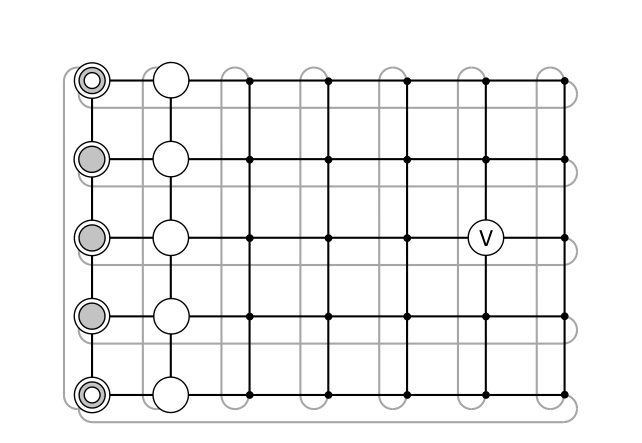
\includegraphics[width=2.8in]{figures/torus1.png}} 
%  \hspace{1in} 
  \subfigure[$t_1$]{ 
    \label{fig:torus2:b} %% label for second subfigure 
    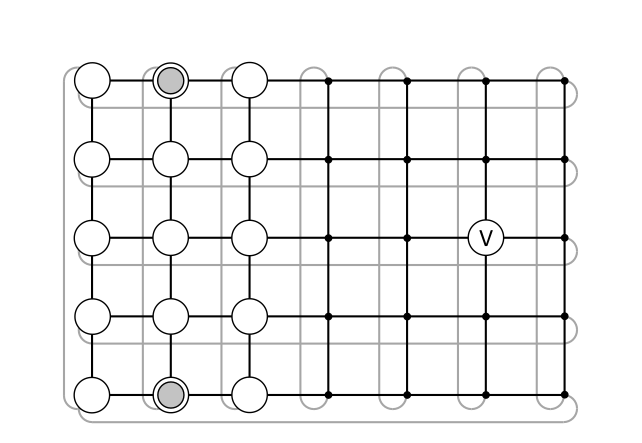
\includegraphics[width=2.8in]{figures/torus2.png}}
    \hspace{1in} 
  \subfigure[$t_2$]{ 
    \label{fig:torus3:c} %% label for second subfigure 
    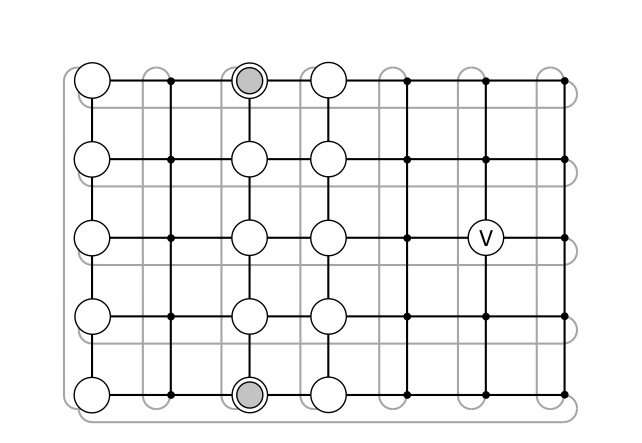
\includegraphics[width=2.8in]{figures/torus3.png}}
%      \hspace{1in} 
  \subfigure[$t_3$]{ 
    \label{fig:torus4:d} %% label for second subfigure 
    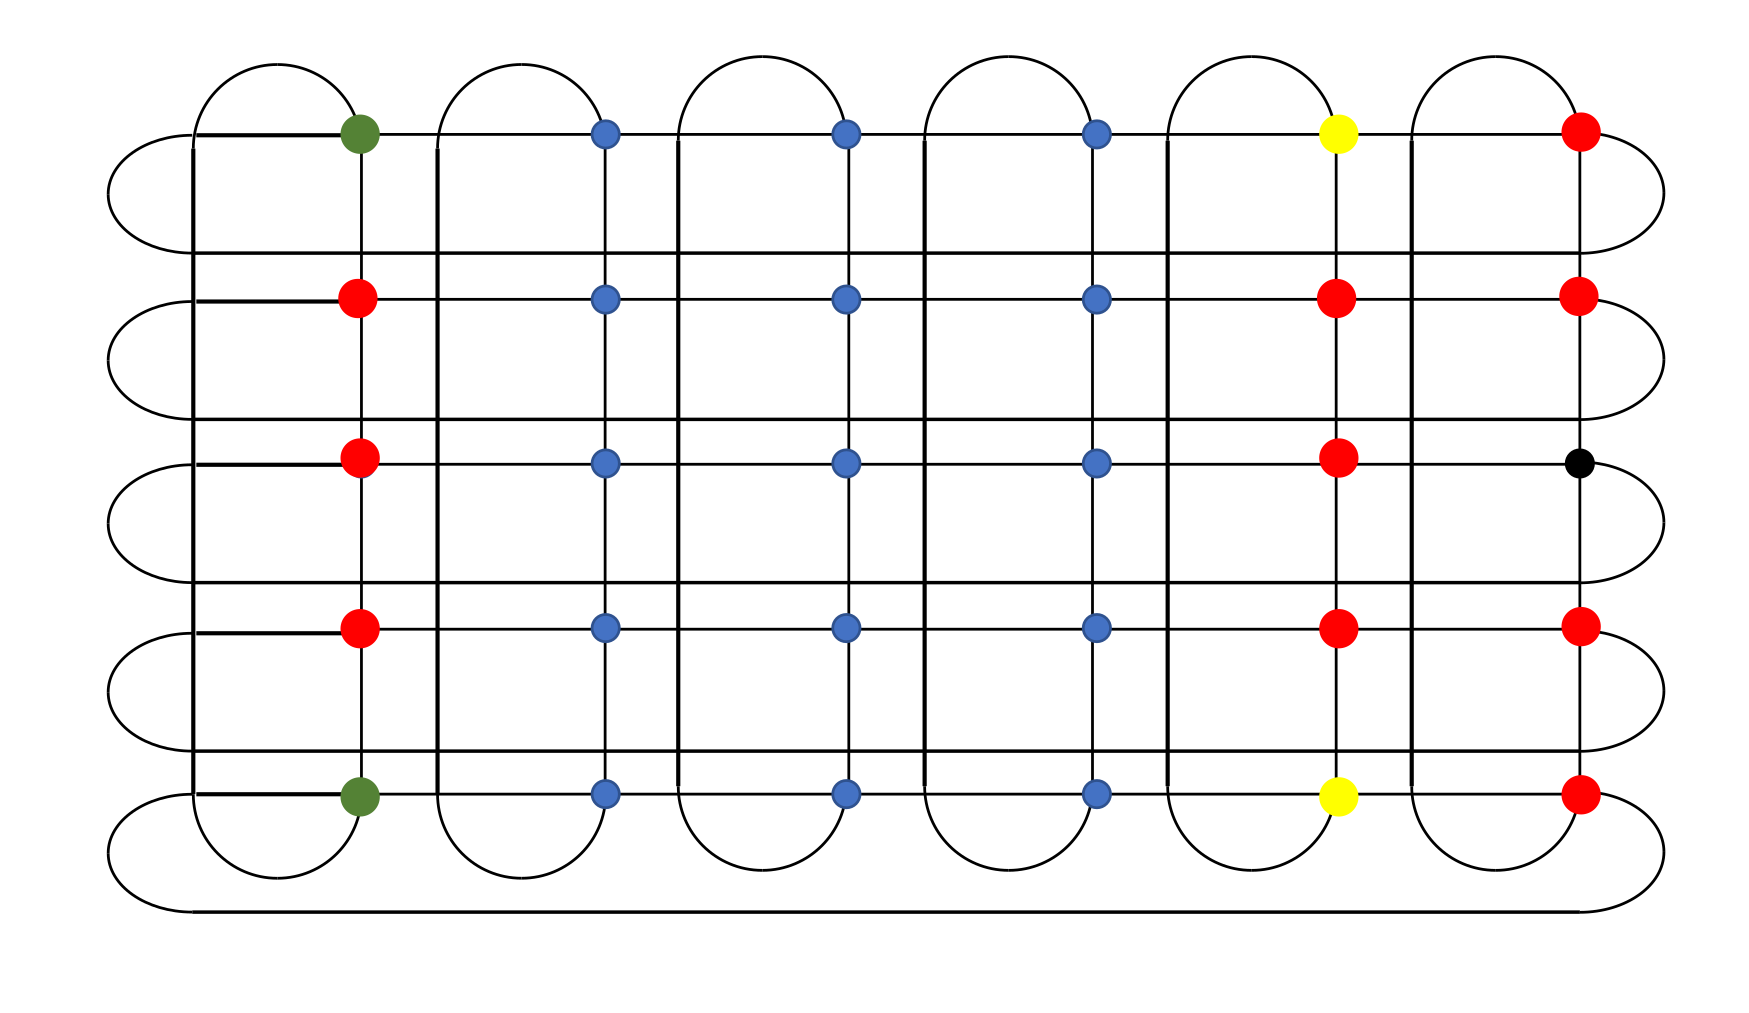
\includegraphics[width=3in]{figures/torus4.png}}
      \hspace{1in} 
  \subfigure[$t_4$]{ 
    \label{fig:torus5:e} %% label for second subfigure 
    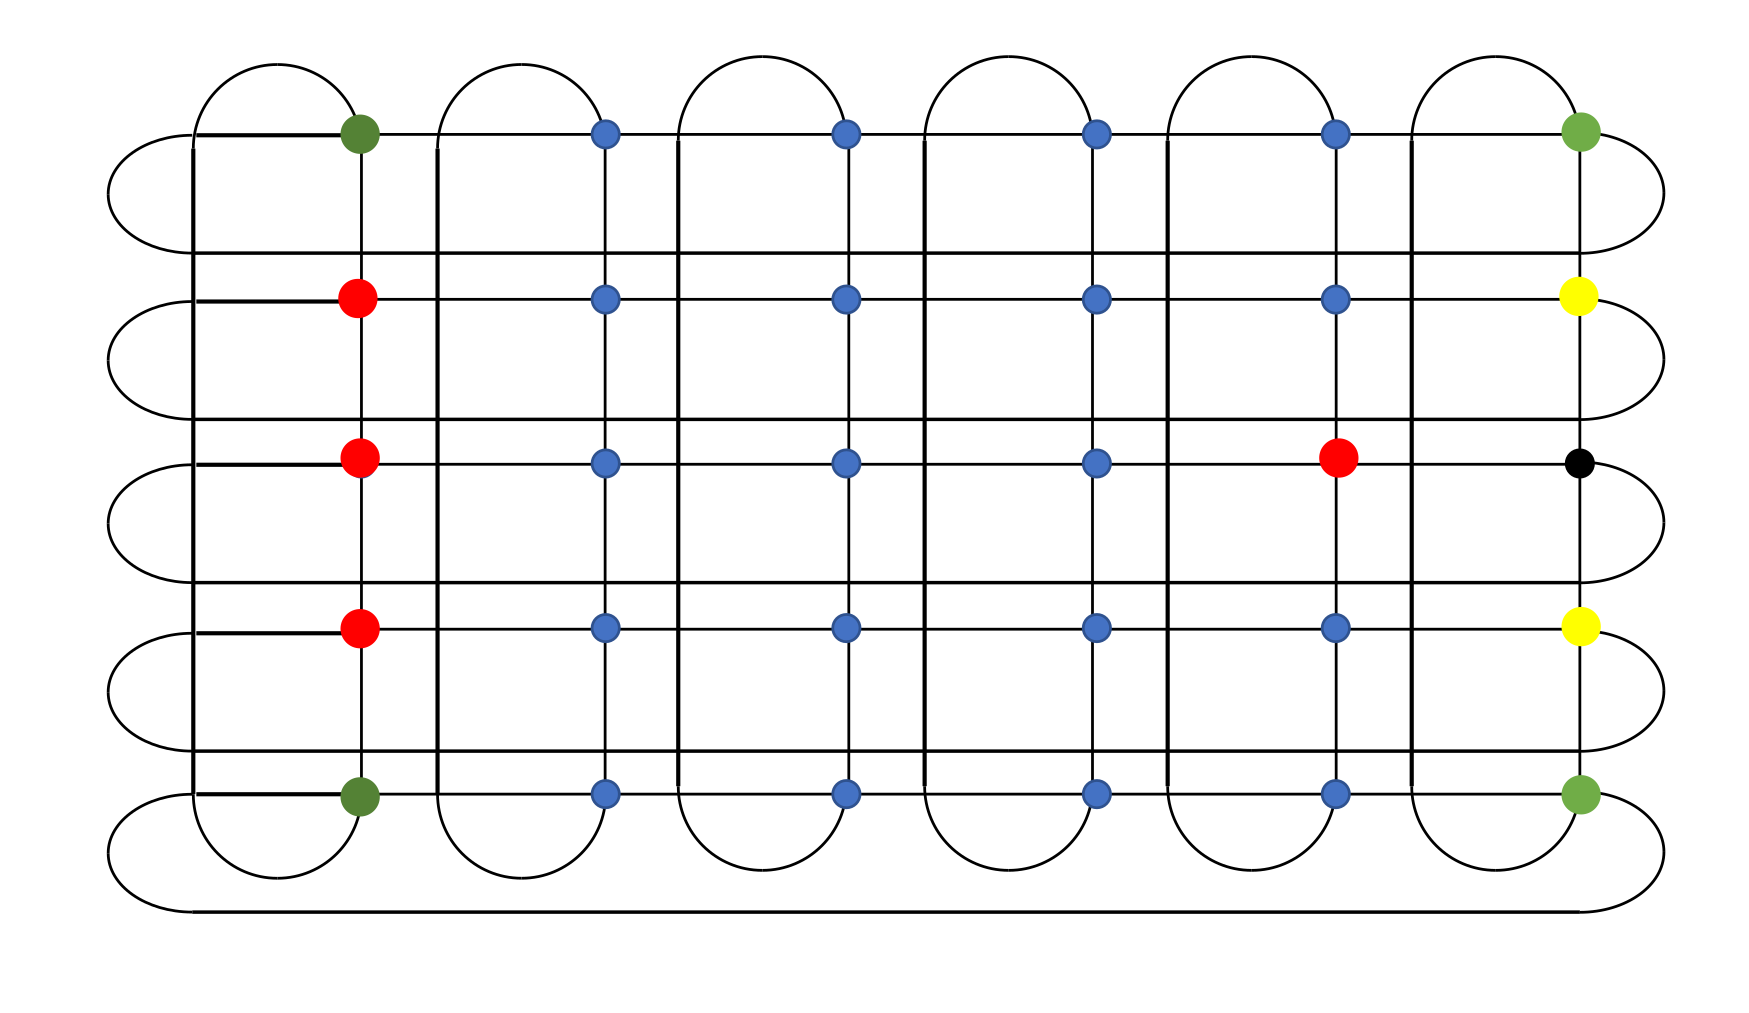
\includegraphics[width=2.8in]{figures/torus5.png}}
     \subfigure[$t_5$]{ 
    \label{fig:torus6:e} %% label for second subfigure 
    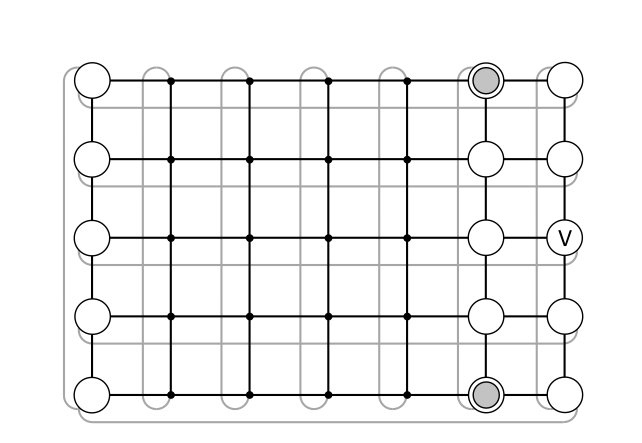
\includegraphics[width=2.8in]{figures/torus6.png}}
    \hspace{1in} 
  \subfigure[$t_6$]{ 
    \label{fig:torus3:c} %% label for second subfigure 
    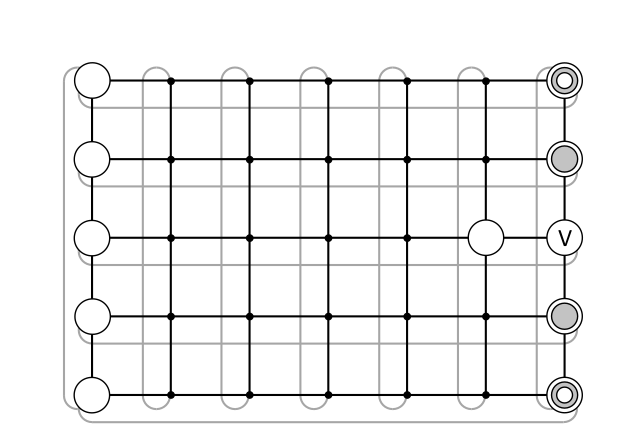
\includegraphics[width=2.8in]{figures/torus7.png}}     
    %\hspace{1in} 
  \subfigure[$t_7$]{ 
    \label{fig:torus4:d} %% label for second subfigure 
    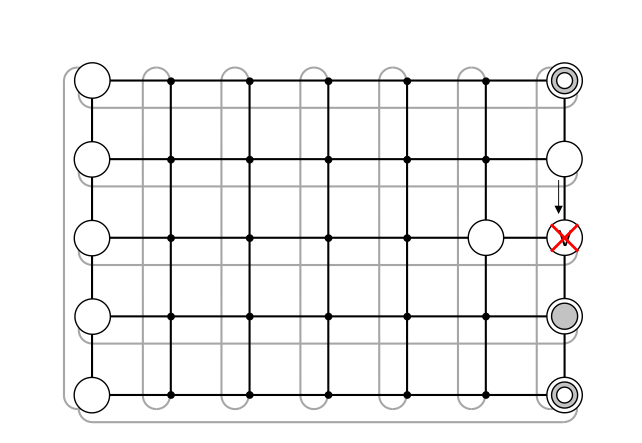
\includegraphics[width=2.8in]{figures/torus8.png}}
  \caption{Arrangement of agents PBVD-T} 
  \label{fig:torus} %% label for entire figure 
\end{figure}
%\fi

Let ${\cal T}$ be a   torus of size   $n=d_1\times d_2(d_1>2,d_2>2)$, with $d_1=min\{ d_1,d_2 \}$.

\begin{theorem}
The PBVD-T performs a decontamination of  ${\cal T}$  using $3d_1+2$ agents (in the worst case, 
$3\sqrt n+2$  agents) and at most 1 casualty,  with at most $2n-\sqrt{n}+O(1)$ movements and at most  time $\sqrt{n}+11$.
\end{theorem}
\begin{proof}
To complete the exploration and the elimination, we need $2(d_1+1)$ agents which has been alsready proven in Theorem 2, plus  $d_1$ agents to guard the first column, so we need in total $3d_1+2$ agents (which is $3\sqrt{n}+2$ in the worst case).  The computation of casualties,  number of movements, and   time   follow from Theorem 2.
\end{proof}


\color{blue}
\section{Summary}
In this chapter, the parallel BVD problems have been examined for two classes of interconnection networks: grids and tori. The parallel decontamination protocols for these two classes have been presented. Agents in our solution use only local information to execute the protocol. A summary (see 
Table \ref{table:Summary of Results of Parallel Strategies in Grids and Toris}  ) of the results is shown in the table below, where $q$ denotes the dimensions of the network, and n denote the numbers of nodes.

\begin{table} [hbtp]
\caption{Summary of Results of Parallel Strategies in Grids and Toris}
\label{table:Summary of Results of Parallel Strategies in Grids and Toris}
\centering
\tabulinesep=2mm
\begin{tabu} to 140 mm {|X[6,c]|X[4,l]|X[4,l]|X[4,l]|X[4,l]|} \hline 
%\begin{tabular}{|c|l|} \hline 
Network  &   Spread &   Size   &   Movements &   Time \\ \hline
{\em 2-Grid}   &1 &$2(\sqrt{n}+1)$& $2n-\sqrt{n}+O(1)$   & $\sqrt{n}+11$         \\ \hline
{\em q-Grid (size of $n=d_1\times\ldots\times d_p\times\ldots\times d_q$)} & $q-p+1$    & $2\times d_1\times\ldots\times d_p (1\leq p\leq q)$  & $O(qn)$      & $\Theta (\frac{n}{d_1\times\ldots\times d_p})$            \\ \hline
{\em 2-Tori} & 1   & $3\sqrt{n}+2$          & $2n-\sqrt{n}+O(1)$     & $\sqrt{n}+11 $    \\ \hline

\end{tabu}
%\end{tabular}
\end{table}


\color{black}














